% Created 2023-05-17 Wed 23:39
% Intended LaTeX compiler: pdflatex
\documentclass[a4paper,12pt]{article}
\usepackage[utf8]{inputenc}
\usepackage[T1]{fontenc}
\usepackage{graphicx}
\usepackage{longtable}
\usepackage{wrapfig}
\usepackage{rotating}
\usepackage[normalem]{ulem}
\usepackage{amsmath}
\usepackage{amssymb}
\usepackage{capt-of}
\usepackage{hyperref}
\usepackage{tikz}
\usepackage{fontspec}
\usepackage{unicode-math}
\usepackage[margin=1.2in]{geometry}
\renewcommand{\baselinestretch}{1.25}
\setlength{\abovedisplayskip}{7pt}
\setlength{\belowdisplayskip}{7pt}
\setlength{\abovedisplayshortskip}{7pt}
\setlength{\belowdisplayshortskip}{7pt}
\setmainfont{Libertinus Serif}
\setmathfont{Libertinus Math}
\date{}
\title{A Comparative Study of Dynamic Linear Models and ARIMA Models for Renewable Energy Forecasting}
\hypersetup{
 pdfauthor={Prashant Tak},
 pdftitle={A Comparative Study of Dynamic Linear Models and ARIMA Models for Renewable Energy Forecasting},
 pdfkeywords={},
 pdfsubject={},
 pdfcreator={Emacs 28.2 (Org mode 9.6.1)}, 
 pdflang={English}}
\begin{document}

\begin{titlepage}
    \begin{center}
        %\vspace*{1cm}
        \Large
        \textbf{A Comparative Study of Dynamic Linear Models and ARIMA Models for Renewable Energy Forecasting}

        \vspace{0.5cm}
        \large
        Thesis \\
        Submitted in partial fulfillment of the requirements of\\
        BITS F424T Thesis \\
        By

        \vspace{0.5cm}

        \textbf{Prashant Tak} \\
        \textbf{(2018B4A81050P)}

        \vspace{0.5cm}
        \vfill

        Under the supervision of\\
        \textbf{Dr. Sumanta Pasari}\\
        Assistant Professor\\
        Department of Mathematics

        \vspace{0.8cm}

        
\includegraphics[width=0.4\textwidth]{bitslogo.pdf}

        \normalsize
        BIRLA INSTITUTE OF TECHNOLOGY AND SCIENCE PILANI\\
        PILANI CAMPUS\\
        Rajasthan - 333031\\
        May 2023

    \end{center}
\end{titlepage}
\pagebreak

\section{Acknowledgement}
\label{sec:orgcfe4dcd}
I would like to thank the Mathematics Department of BITS Pilani for providing me with this incredible opportunity to pursue my undergraduate thesis and for providing me with the background necessary to start working on the project.

I'd also like to thank Dr. Sumanta Pasari who has guided me in the whole endeavour from the beginning. At every step, he has provided me with valuable inputs and motivation to do better. Alongwith that, I'd also like to mention Ms. Sakshi Shukla, who has provided me with suggestions regarding through the whole process and clarified any doubts I had.

Last but not the least, I would like to thank my parents for providing me with lessons throughout my life and never ending moral and financial support.
\pagebreak

\thispagestyle{plain}
\begin{center}
    \large
    \textbf{CERTIFICATE}\\
\end{center}
This is to certify that the Thesis entitled, \emph{A Comparative Study of Dynamic Linear Models and ARIMA Models for Renwable Energy Forecating} and submitted by \emph{Prashant Tak} ID No. \emph{2018B4A81050P} in partial fulfillment of the requirement of BITS F424T Thesis embodies the work done by him under my supervision.\\
\vspace{1.5cm}\\
Date:\hspace*{\fill}Dr. Sumanta Pasari\\
\hspace*{\fill}Assistant Professor\\
\hspace*{\fill}Department of Mathematics\\
\hspace*{\fill}BITS Pilani, Pilani Campus\\
\pagebreak

\tableofcontents \clearpage

\section{Abstract}
\label{sec:org0fefb02}
Short-term energy forecasting influences energy plants operations a lot and it can also have environmental impact. This report looks into studying Dynamic Linear Models for assessing solar irradiance and wind speed values and estimating them. The Global Horizontal Irradiance (GHI) data for Bhadla Solar Park (Gujarat) from 2001 to 2021 is considered for the analysis. For wind speed, data from numerous locations over India is looked at. The analysis is done with short-term(daily), mid-term(weekly) and long-term(monthly) data. The stationarity of the data is verified using ADF test and a dynamic linear regressive framework with seasonal terms is proposed to model the GHI values. The parameters for the model are obtained via Kalman Filter. The predictions are compared with ARIMA and Seasonal ARIMA models. The residuals for the predicted values are investigated using Shapiro-Wilk test and Q-Q plots.
\pagebreak

\section{Introduction}
\label{sec:orgadedeb2}
A country's ability to advance economically and technologically is greatly influenced by its access to electricity. The amount of power produced globally has significantly increased as a result of society's growing reliance on energy. Conventional fossil fuels are frequently the main contributors to the production of electricity globally. They take a long time to create, and the rate at which current reserves are being used up is much higher than the rate at which they are being produced. As a result, they are close to going extinct.

Fossil fuels are also one of the main sources of greenhouse gas emissions, which significantly contribute to global warming and, as a result, pose a threat to the environment and human-dependent living conditions. In recent years, the emphasis has shifted from the use of fossil fuels to the use of renewable energy sources for the production of electricity. Accurate renewable energy forecasting aids in planning and projecting energy output from the short to the long term.

The contribution of wind and solar energy is notable among other renewable energy sources. For a variety of practical uses, including estimating plant energy outputs, marketing renewable energy, and planning maintenance for wind farms and solar plants, wind speed and GHI estimates are helpful. While monthly weather forecasts can be utilised for long-term planning of power plants, daily forecasts can be used to determine the optimal months for solar and wind energy production.

GHI (Global Horizontal Irradiance) refers to the amount of radiant power from sunlight received by a particular surface, perpendicular to the sun’s rays. It is useful when monitoring a solar power plant, finding optimal placement location of solar plants and for assessing solar power plant feasibility. The higher the GHI value, the more power a system will produce. Its measurement unit is Watts per Sq Meter (W/m\textsuperscript{2}).

Wind speed data can be used for analysing areas and periods of large wind-speed and wind mills could be installed and activated in those regions for renewable energy sourcing. Short term predictions are generally used for real-time monitoring, whereas weekly forecasts can be utilized for scheduling maintenance of the existing systems.

One early work on DLMs is the seminal paper by West and Harrison (1997), which introduced the general form of the model and its estimation using the Kalman filter. They demonstrated the flexibility of the DLM framework through a series of examples, including trend, seasonal, and autoregressive models. Their work has been influential in the development of DLMs for forecasting.

In finance, DLMs have been used to model and forecast asset returns and volatility. For example, Cogley and Sargent (2005) applied a DLM with stochastic volatility to forecast equity premium, and Liu et al. (2019) used a DLM with time-varying volatility to forecast Bitcoin returns. In economics, DLMs have been used to forecast macroeconomic variables such as GDP, inflation, and unemployment. For instance, Primiceri (2005) used a DLM with stochastic volatility to forecast inflation, and Chan and Koop (2013) used a DLM with time-varying coefficients to forecast US GDP. DLMs have also been applied to engineering problems such as signal processing and control. For example, Yang et al. (2018) used a DLM to forecast solar power generation, and Jiang et al. (2019) used a DLM to control the positioning of a linear motor. These models can capture the dynamics of physical systems and provide accurate forecasts for future behavior.

Wang et al. (2019) used Bayesian DLMs to predict and model temprature-caused strain of a long-span bridge whereas Khan and Firdos (2021) used DLMs to forecast infections, deaths and recovery numbers in Pakistan due to Covid-19. Wang (2017) has also used Bayesian methods for health evaluation by data monitoring.
\pagebreak
\section{Background Literature}
\label{sec:org06f8061}
Statistical analysis of time series data is usually faced with the problem that we have only one realization of a process whose properties we might not fully understand. A Dynamic Linear Model (DLM) is a time series forecasting method that combines linear regression with a state-space model. It allows for modeling time-varying parameters and can incorporate both exogenous variables and latent variables that are unobserved but influence the time series. The key advantage of DLM over other forecasting methods is its ability to model time-varying parameters, which makes it suitable for modeling complex dynamic systems. In linear trend analysis, we assume that there is an underlying change in the background that stays approximately constant over time. In dynamic regression systems, by explicitly allowing for variability in the regression coefficients we let the system properties change in time. Also, unlike ARMA models, they can be applied to non-stationary data without transformation. Furthermore, the use of unobservable state variables allows direct modelling of the processes that are driving the observed variability, such as seasonality or external forcing, and we can explicitly allow for some modelling error.
\subsection{Bayesian Inference}
\label{sec:org63b7cb3}
Bayesian inference is a statistical approach to data analysis and decision making that involves updating probabilities based on new data and prior knowledge. In Bayesian inference, probabilities are treated as measures of uncertainty rather than frequencies. The key idea is to start with an initial prior probability distribution that represents our beliefs about the unknown parameters of interest, and then update this distribution based on observed data using Bayes' theorem. It states that
\[
  Posterior = \frac{Likelihood * Prior}{Evidence}
\]
Bayesian inference allows for incorporating prior knowledge or assumptions about the parameters, which can improve the estimation and prediction accuracy.
\subsection{Dynamic Linear Models}
\label{sec:org3c267f3}
State space models consider a time series as the output of a dynamic system perturbed by random disturbances. They allow a natural interpretation of a time series as combination of trend, seasonal or regressive components. In a state space model we assume that there is an unobservable Markov chain (x\textsubscript{t}), called the \emph{state process}, and that y\textsubscript{t} is an \emph{imprecise measurement} of x\textsubscript{t}. A trivial DLM consists of two sets of equations:
\[
y_{t} = F_{t}x_{t} + v_{t}
\]
\[
x_{t} = G_{t}x_{t-1} + w_{t}
\]
Here y\textsubscript{t} represents the observation at time t, v\textsubscript{t} and w\textsubscript{t} are sequences of independent gaussian random errors (\emph{observation error and evolution error}) and x\textsubscript{t} corresponds to the unobserved state of the system having a \emph{prior distribution} for \(x_{0} \sim N(m_{0}, C_{0})\). F\textsubscript{t} and G\textsubscript{t} are the \emph{observation} and \emph{system matrices}.
\subsection{Kalman Filters}
\label{sec:org66792b1}
Model building can be a major difficulty: there might be no clear identification of physically interpretable states, or the state space representation could be non unique, or unsuitable choice of parameters could result in an inadequate model. To estimate the state vector we compute the conditional densities \(\pi(x_{s}|y_{1:t})\). We distinguish between problems of filtering (when s = t), state prediction (s > t) and smoothing (s < t).

In a DLM, the Kalman filter provides the formula for updating our current inference on the state vector as new data become available, that is, for passing from the filtering density \(\pi(x_{1}|y_{1:t})\) to \(\pi(x_{t+1}|y_{1:t+1})\). It allows us to compute the predictive and filtering distributions recursively, starting from \(x_{0} \sim N(m_{0}, C_{0})\) then computing \(\pi(x_{1}|y_{1})\), and proceeding recursively as new data becomes available. This is the usual Bayesian sequential updating, in which the posterior at time t takes the role of a prior distribution for what concerns the observations after time t.
\subsubsection{Filtering}
\label{sec:org40e7a21}
Taking the vector of observations y\textsubscript{1:t}, the filtering distribution \(\pi(x_{t}|y_{1:t})\) is computed recursively as:
\begin{enumerate}
\item Start with \(x_{0} \sim N(m_{0}, C_{0})\)
\item One step forecast for the \emph{state}:
\[
    x_{t}|y_{1:t} \sim N(a_{t}, R_{t})\ \text{where}\ a_{t} = G_{t}m_{t-1}\ \text{and}\ R_{t} = (G_{t}C_{t-1}G'_{t}) + W_{t}
   \]
\item One step forecast for the \emph{observation}:
\[
    y_{t}|y_{1:t} ~ N(f_{t}, Q_{t})\ \text{where}\ f_{t} = F_{t}a_{t}\ \text{and}\ Q_{t} = (F_{t}R_{t-1}F'_{t}) + V_{t}
   \]
\item Compute the posterior at time t:
\[
    x_{t} | y_{1:t} \sim N(m_{t}, C_{t})\ \text{where}\ m_{t} = a_{t}+R_{t}f'_{t}Q^{-1}_{t}(y_{t}-f_{t})\ \text{and}\ C_{t} = R_{t} - (R_{t}F'_{t}Q^{-1}_{t}F_{t}R_{t})
   \]
\end{enumerate}
\pagebreak
\subsubsection{Forecasting}
\label{sec:org0fc433f}
To calculate forecast distributions, for k = 1, 2 \ldots{}
\begin{enumerate}
\item Start with a sample from \(x_{T} | y_{T} \sim N(m_{T}, C_{T})\)
\item Forecast the state:
\[
            x_{T+k} | y_{1:T} \sim N(a_{k}^T, R_{k}^T)\ \text{where}\ a_{t}^k = G_{T+k}a^{T}_{k-1}\ \text{and}\ R_{k}^T = G_{T+k}R^{T}_{k-1}G'_{T+k} + W_{T+k}
    \]
\item Forecast the observation:
\[
            y_{T+k} | y_{1:T} \sim N(f_{k}^T, Q_{k}^T)\ \text{where}\ f_{t}^k = F_{T+k}a^{T}_{k-1}\ \text{and}\ Q_{k}^T = F_{T+k}R^{T}_{k-1}F'_{T+k} + V_{T+k}
         \]
\end{enumerate}
\subsection{ARIMA \& Seasonal ARIMA}
\label{sec:org69d46a8}
\subsubsection{From AR to ARIMA}
\label{sec:org7447969}
\begin{itemize}
\item Auto-Regressive (AR) models, as the name suggests makes the predictions by taking into consideration previous values, the number of previous values it uses is defined by the order \emph{p}. Thus the model equation is given by:
\[
    X_{t} = \sum_{i=1}^{p} a_{i}x_{t-i} + \omega_{t}
  \]
where a\textsubscript{i}s are the model coefficients and \(\omega\)\textsubscript{t} is noise.
\item Moving Average (MA) models express the present value as a linear combination of the mean of the series, the present error term and the past error terms. The model is denoted by:
\[
    X_{t} = \mu + \epsilon_{t} + \sum_{j=1}^{q} \theta_{j} \epsilon_{t-j}
  \]
where \(\theta\)\textsubscript{i}s are the associated coefficients, \(\mu\) is the time series mean and \(\epsilon\)\textsubscript{t} is the current error. MA models allow for smoothening the impact of outliers.
\item An ARMA model is just a linear combination of the two containing terms related to the past error terms, previous data values and the current error term.
\item For non-stationary data, ARIMA models are preferred over ARMA models since they perform an additional operation of differencing for non-stationary series allowing it to become stationary. Thus an ARIMA model can be defined by a triplet of parameters called its order referring to \emph{p}, the order referencing the AR term; \emph{q} related to the underlying MA process and \emph{d} that shows the amount of differencing, hence its complete order is \emph{(p, d, q)}.
\end{itemize}
\subsubsection{SARIMA (Seasonal ARIMA)}
\label{sec:orgb4c6bfd}
Seasonality in a time series is a regular pattern of changes that repeats over \emph{T} time periods, where \emph{T} denotes the number of time periods after which the pattern repeats again. In a seasonal ARIMA model, seasonal AR and MA terms predict using data values and errors at times with lags that are multiples of \emph{T} (the span of the seasonality). A seasonal ARIMA model incorporates both seasonal and non-seasonal ARIMA models in a multiplicative fashion.
\[
  ARIMA(p, d, q) \times (P, D, Q)_{S}
\]
the order (P, D, Q) refers to the seasonal order of the model.
\subsubsection{Advantages and Disadvantages}
\label{sec:org5a4b367}
Implementation of these models is quite trivial and they can be used on a wide array of time-series. However for long seasonal periods, SARIMA models fail to perform well due to large amount of memory consumption and complex dependencies in the data. They also are relatively inaccurate when it comes to non-linear relationships in the data.
\subsection{Model Evaluation}
\label{sec:orgf7b130d}
Once a time series model makes its forecasts, analysing the nature and accuracy of those predictions becomes the next step. There are numerous ways of measuring a model but we'll consider the most standard ones related to prediction errors. The lower the value, the better a model's prediction.
\subsubsection{Root Mean Squared Error (RMSE)}
\label{sec:org2d5d48c}
RMSE, the standard deviation of the residuals shows how much of the data is centered (gathered) around the best fit line. It quantifies the spread of forecast error values.
\[
  RMSE = \sqrt{\frac{1}{N}\sum_{i=1}^N (y_{i, actual} - y_{i, predicted})^{2}}
\]
\subsubsection{Mean Absolute Error (MAE)}
\label{sec:org2e88f1a}
It is a measure of the absolute difference between the forecasted and the real value. It does not provide any weight to the errors unlike RMSE but rises linearly with the errors.
\[
  MAE = \frac{1}{N}\sum_{i=1}^{N} | (y_{i, actual} - y_{i, predicted}) |
\]
\subsubsection{Mean Absolute Percentage Error (MAPE)}
\label{sec:orgd3faa92}
It standardises the value of each error term by dividing it with the actual value.
\[
  MAPE = \frac{1}{N}\sum_{i=1}^{N} \frac{(y_{i, actual} - y_{i, predicted})}{y_{i, actual}}
\]
\subsection{Residual Analysis}
\label{sec:org43a76d8}
The residuals are the error values for the predicted data. For checking whether or not there is any bias present in the implemented models, analysing the residuals of the predictions is a necessary step. The residuals should exhibit normal gaussian distribution with zero mean and a constant variance. To test the normality of the residuals, one can use the Shapiro-Wilk test. It tests the null hypothesis that a sample came from a normal distribution, hence if the p-value is less than 0.05 (95 \% confidence level) then the null hypothesis is rejected and the residuals are not considered as normally distributed.

But for large sample sizes, it over estimates even simple deviations from the null hypothesis thus an additional analysis using Q-Q plots can be done. If the two distributions that are compared are similar then points on the Q-Q plot lie along the \emph{y = x} line. If one of the ends of the Q-Q plot deviates from the straight line, it is an indicator of skewness in the sample. An \emph{n\textsuperscript{th}} quantile means that n\% of the data falls below that point.
\pagebreak
\section{Formulation and Methodology}
\label{sec:orgf8ffe0f}
For estimation of the GHI and Wind Speed values, a Linear Regressive Dynamic Model is chosen with seasonal factors. A linear regression model (with lagged values of observation as regression variable) looks like
\[
y_{t} = y_{t-1}x_{t} + v_{t}
\]
\[
x_{t} = G_{t}x_{t-1} + w_{t}
\]
The available data for GHI and wind speed (for Tiruvanantpuram) are hourly data without a date-time index. Therefore, a date-time index for the data is created and any missing values are dealt with. Because of the large volume of data, it is resampled to monthly and weekly values to allow for model fitting. Due to the absence of sun radiation, values from night-time to early morning are minimal in GHI data. Therefore, those values are omitted, as the forecast is only necessary for times when there is sufficient sun irradiation. The wind speed data for rest of the locations is resampled to daily data for analysis.

Then, the Augmented Dickey-Fuller(ADF) test is run to determine whether the time series is stationary or not. The null hypothesis of the ADF is that the underlying series is nonstationary, whereas the alternative hypothesis is that the series is stationary but lacks a unit root. If the p-value of the ADF test is less than the critical value, then the data is considered stationary. When p-values are large, however, the null hypothesis cannot be rejected, indicating that the data is not stationary.

Afterwards, the time series is decomposed using an additive model (since it has no trend with respect to time) into trend, seasonality and residuals. This allows one to infer about the underlying characteristics of the data and provides initial ideas regarding the formulation of the DLM. The data for all the analysis was procured from National Solar Radiation Database (NSRDB) maintained by the \href{https://nsrdb.nrel.gov/}{U.S. Department of Energy}.

The DLM implementation is performed with the help of \texttt{pyDLM} library. The DLM is built upon two layers. The first layer is the fitting algorithm. DLM adopts a modified Kalman filter with a unique discounting technique from Harrison and West (1999). The second layer of DLM is its modeling feature. The DLM can easily incorporate most modeling components and turn them into the corresponding transition matrices and other quantities to be supplied to the Kalman filter. Examples are trend, seasonality, holidays, control variables and auto-regressive, which could appear simultaneously in one model.

For the analysis here, two different DLM models are constructed, one containing only seasonal and trend components which results in a very periodic predictive model and another that is supplied with an additional lagged regressive component. The second model is dynamic that can incorporate sudden non-linearities.

For getting the order for the ARIMA and SARIMA models, different paths were taken. The ideal order value for ARIMA was found using the grid-search method that enumerates all possible combinations of the order and picks the one with the least RMSE value. For obtaining the order for SARIMA model, the \texttt{auto.arima} function was leveraged which computes the AIC criterion for each chosen order and picks the one with the least AIC value.

After creating the Regressive model (with lagged values of data) and Seasonal model and applying the Kalman Filter, the estimated plots are generated and the residuals are computed and analysed using Shapiro-Wilk test to measure the residuals' normality. \\[0pt]

\usetikzlibrary{shapes.geometric, arrows}
\tikzstyle{startstop} = [rectangle, rounded corners,
minimum width=3cm,
minimum height=1cm,
text centered,
draw=black,
fill=red!30]
\tikzstyle{io} = [trapezium,
trapezium stretches=true, % A later addition
trapezium left angle=60,
trapezium right angle=120,
minimum width=3cm,
minimum height=1cm, text centered,
draw=black, fill=blue!30]
\tikzstyle{decision} = [diamond,
minimum width=3cm,
minimum height=1cm,
text centered,
draw=black,
fill=green!30]
\tikzstyle{arrow} = [thick,->,>=stealth]
\begin{tikzpicture}[node distance=3cm]
\node (decomp) [io] {Time Series Decomposition};
\node (ADF) [decision, below of=decomp] {ADF Test};
\draw [arrow] (decomp) -- (ADF);
\node (fail) [startstop, right of=ADF, xshift=4cm] {Non-Stationary Series};
\draw [arrow] (ADF) -- node[anchor=south] {p > 0.05} (fail);
\node (dlm) [io, below of=ADF] {DLM};
\node (arima) [io, below of=ADF, xshift=4cm] {ARIMA};
\node (sarima) [io, below of=ADF, xshift=-4cm] {SARIMA};
\draw [arrow] (ADF) -- node[anchor=east, rotate=36, xshift=1.4cm, yshift=0.5cm] {not daily data} (sarima);
\draw [arrow] (ADF) -- node[anchor=west] {all data} (dlm);
\draw [arrow] (ADF) -- node[anchor=west, rotate=-36, xshift=-0.5cm, yshift=0.5cm] {all data} (arima);
\node (norm) [decision, below of=dlm] {Shapiro-Wilk};
\path[arrow] {[->] (dlm) edge (norm)
                   (arima) edge (norm)
                   (sarima) edge (norm) };
\node (fail2) [startstop, right of=norm, xshift=4cm] {Non Gaussian Residuals};
\draw [arrow] (norm) -- node[anchor=south] {p < 0.05} (fail2);
\end{tikzpicture}

\pagebreak
\section{Discussion}
\label{sec:org16075b7}
\subsection{Bhadla}
\label{sec:orgb0cb52d}
The dataset for Bhadla is hourly data for 20 years. Because of the absence or lack of sun radiation, values from night-time to early morning are negligible so data only from hour 7 to hour 17 is taken into consideration. The huge data is then resampled based on mean values using python's resampling function into monthly and weekly values.
\subsubsection{Monthly}
\label{sec:org56e9f3f}
Looking at the \texttt{decomposition} of the monthly resampled data, we sense a clear seasonality whereas there's no real trend component.

\begin{figure}[htbp]
\centering
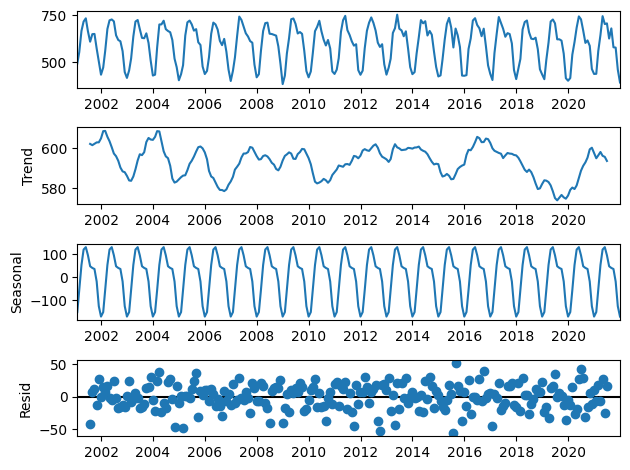
\includegraphics[width=1.00\textwidth]{./images/bhadla/monthlyDecomp.png}
Monthly GHI Decomposition
\end{figure}

Upon constructing the dynamic regressive and seasonal DLM models, their decomposed components are then fitted.

\begin{center}
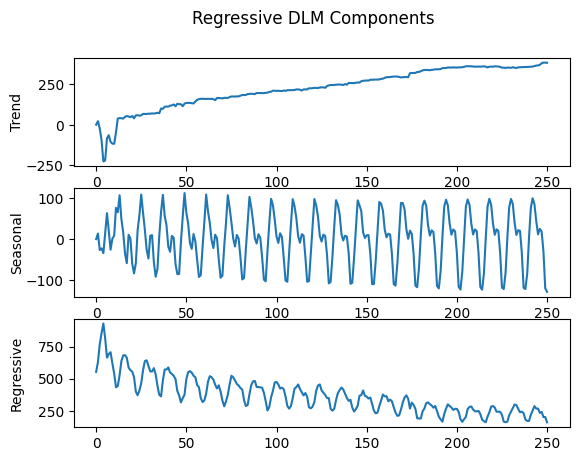
\includegraphics[width=0.7\linewidth]{./images/bhadla/monthlyRegDecomp.png}
\end{center}

\begin{center}
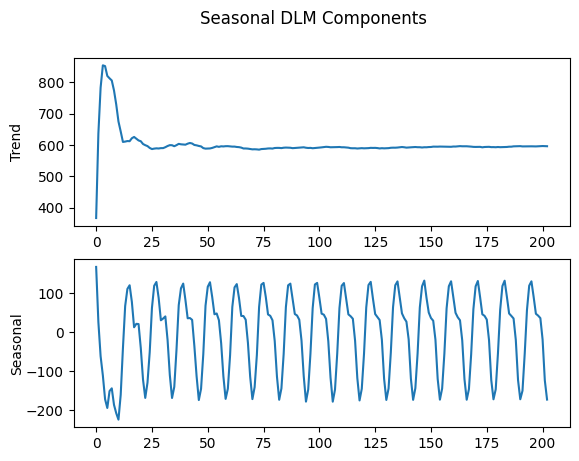
\includegraphics[width=0.7\linewidth]{./images/bhadla/monthlySeasDecomp.png}
\end{center}

Now, taking a look at the predictions for the various models, it's quite evident that ARIMA is performing very poorly whereas the regressive DLM model provides the best fit.

\begin{center}
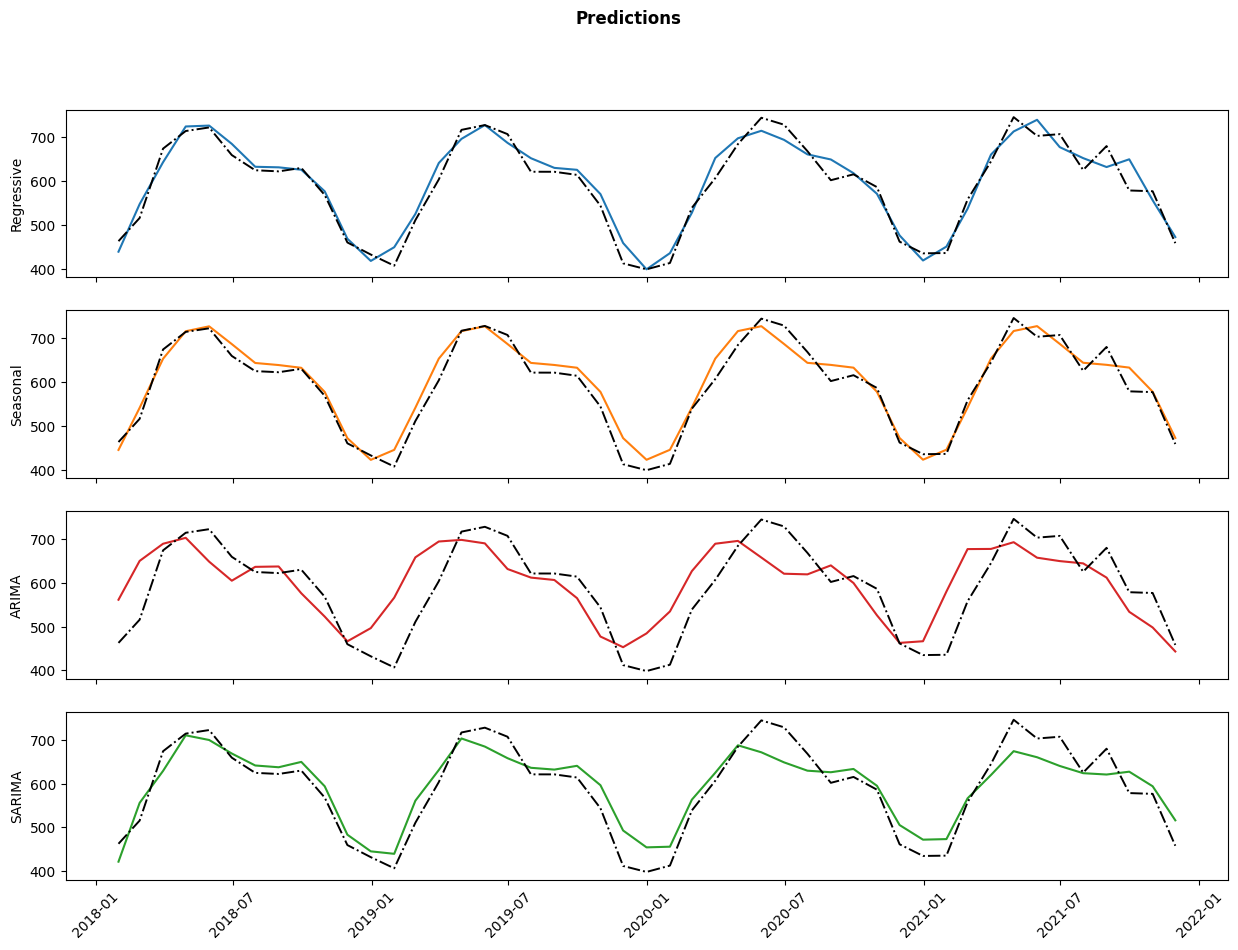
\includegraphics[width=1.00\textwidth]{./images/bhadla/monthlyPred.png}
\end{center}

Looking at the generated residuals and their distribution, the initial observation is confirmed.

\begin{center}
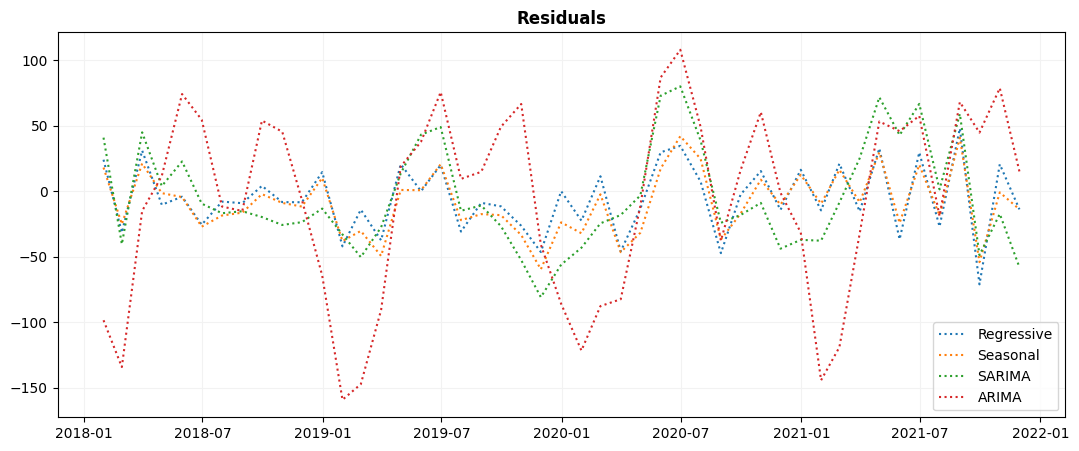
\includegraphics[width=1.00\textwidth]{./images/bhadla/monthlyResid.png}
\end{center}

\begin{center}
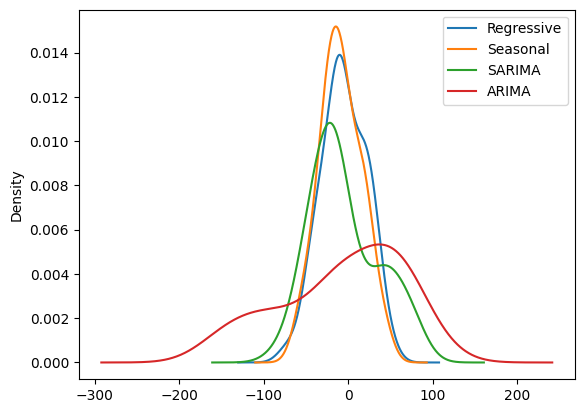
\includegraphics[width=0.8\linewidth]{./images/bhadla/monthlyDist.png}
\end{center}

Taking a look at the Q-Q plots, one can observe that the SARIMA and ARIMA models deviate quite a bit from the y=x line.

\begin{center}
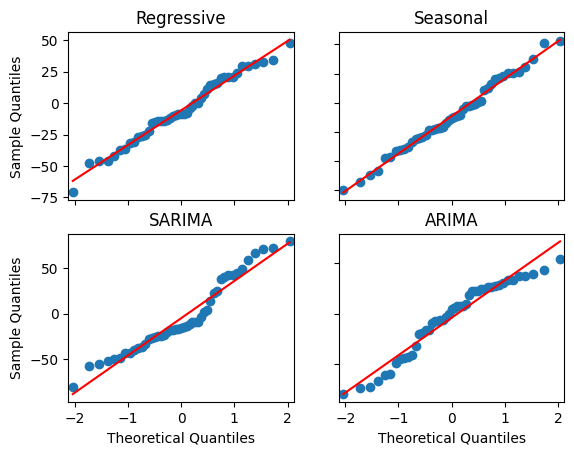
\includegraphics[width=0.8\linewidth]{./images/bhadla/monthlyQQ.png}
\end{center}
\pagebreak

\subsubsection{Weekly}
\label{sec:org4041749}
Now let's take a look at the \texttt{decomposition} of the weekly GHI data, again the pattern repeats, seasonal data with no clear trend.

\begin{figure}[htbp]
\centering
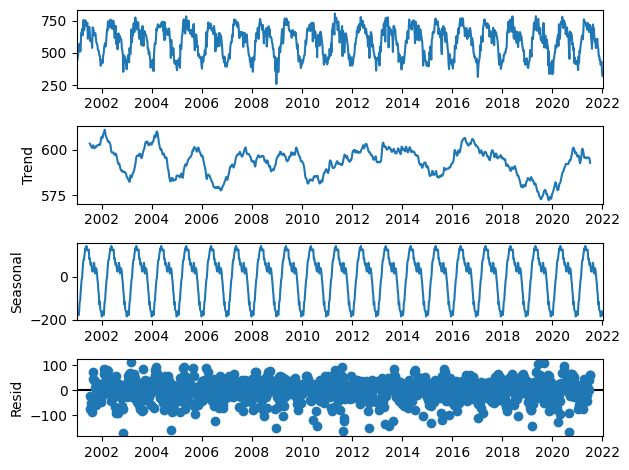
\includegraphics[width=1.0\textwidth]{./images/bhadla/weeklyDecomp.png}
Weekly GHI Decomposition
\end{figure}

The decomposed components for the Regressive and Seasonal DLM models are fitted, they show similar trend and seasonal variations.

\begin{center}
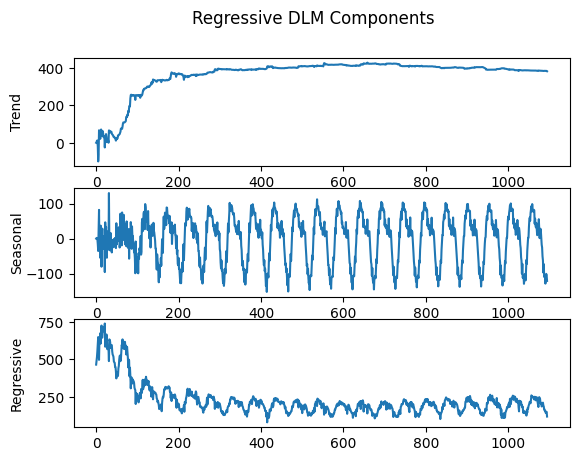
\includegraphics[width=0.45\linewidth]{./images/bhadla/weeklyRegDecomp.png}
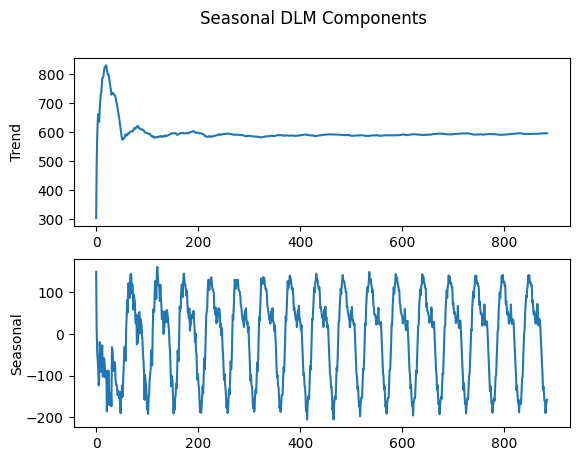
\includegraphics[width=0.45\linewidth]{./images/bhadla/weeklySeasDecomp.png}
\end{center}

From a visual glance at the predictions for the various models, it's not very clear which model's fitting the best, one would have to look at the prediction errors.

\begin{center}
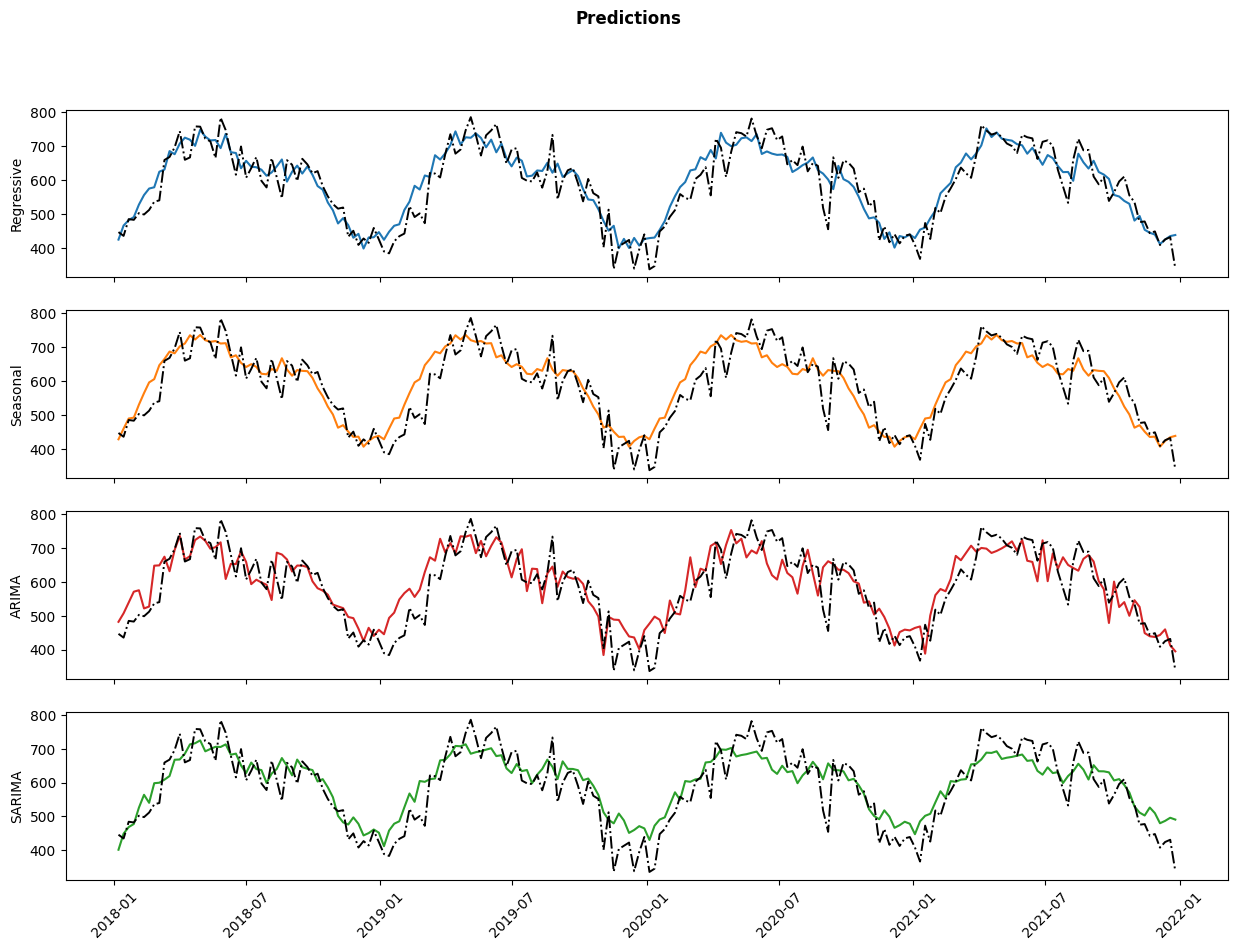
\includegraphics[width=1.00\textwidth]{./images/bhadla/weeklyPred.png}
\end{center}

Even the residuals look quite random and normally distributed.

\begin{center}
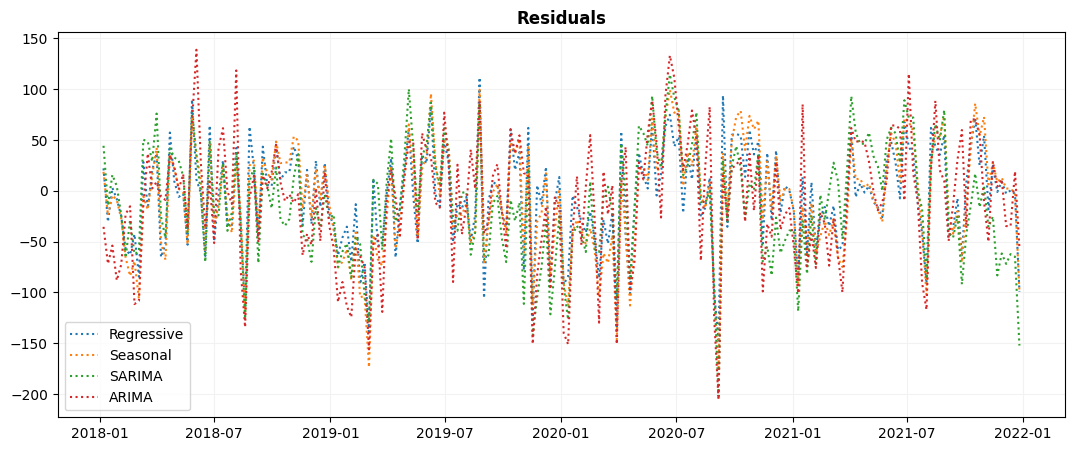
\includegraphics[width=1.00\textwidth]{./images/bhadla/weeklyResid.png}
\end{center}

\begin{center}
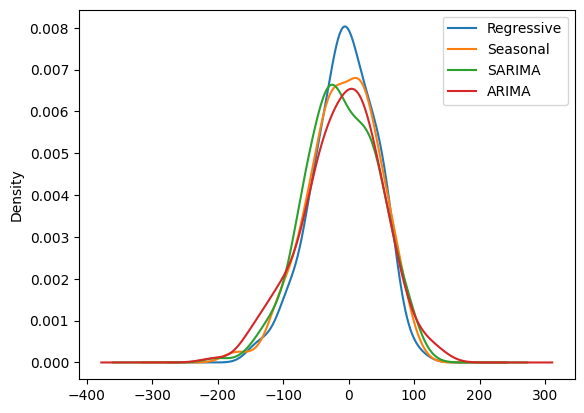
\includegraphics[width=0.8\linewidth]{./images/bhadla/weeklyDist.png}
\end{center}

The Q-Q plots reinforce the same suggestion, for all the models except maybe the seasonal DLM, they follow the \emph{y = x} line.

\begin{center}
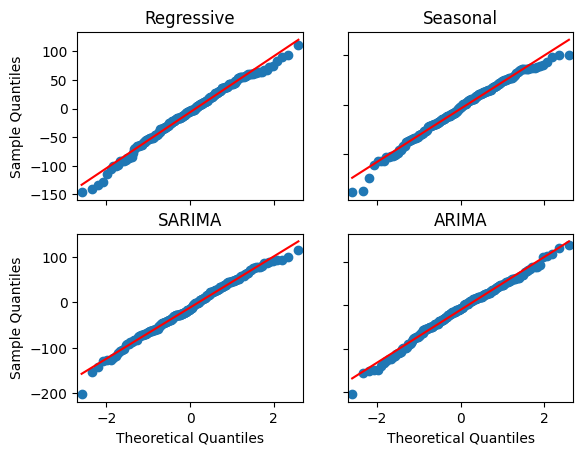
\includegraphics[width=0.8\linewidth]{./images/bhadla/weeklyQQ.png}
\end{center}
\pagebreak
\subsection{Tiruvananthpuram}
\label{sec:org6be26f3}
The data for Tiruvananthpuram for wind speed is of 10 years for monthly and weekly resamples, however for daily data due to resource constraints only 6 years' worth of data is considered. And while the testing data started from 2018 for monthly and weekly data, for daily data it starts from 2019 to allow for a bit more training.
\subsubsection{Monthly}
\label{sec:org0d54bd9}
Looking at the \texttt{decomposition} of the monthly resampled data, we sense a clear seasonality in the data with a small spike at the beginning of each year followed by a large one.

\begin{figure}[htbp]
\centering
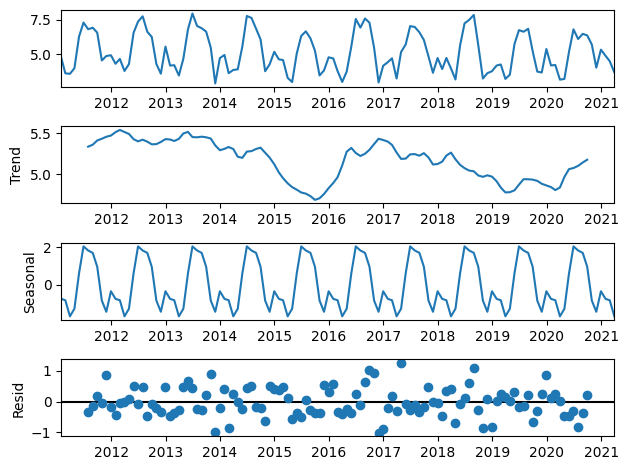
\includegraphics[width=1.00\textwidth]{./images/tiru/monthlyDecomp.png}
Monthly Wind Speed Decomposition
\end{figure}

Upon constructing the dynamic regressive and seasonal DLM models, their decomposed components are then fitted, they show similar characteristics to the decomposed variations.

\begin{center}
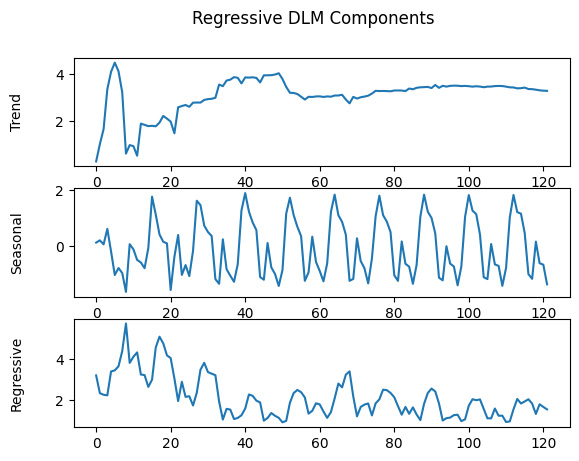
\includegraphics[width=0.7\linewidth]{./images/tiru/monthlyRegDecomp.png}
\end{center}

\begin{center}
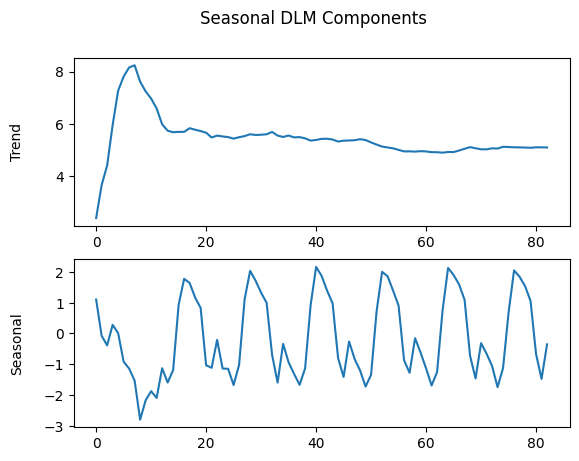
\includegraphics[width=0.7\linewidth]{./images/tiru/monthlySeasDecomp.png}
\end{center}

Now, taking a look at the predictions for the various models, it's quite evident that ARIMA is performing very poorly (later attributed to non-stationarity of the series) whereas the other three models provide a very similar and comparable fit.

\begin{center}
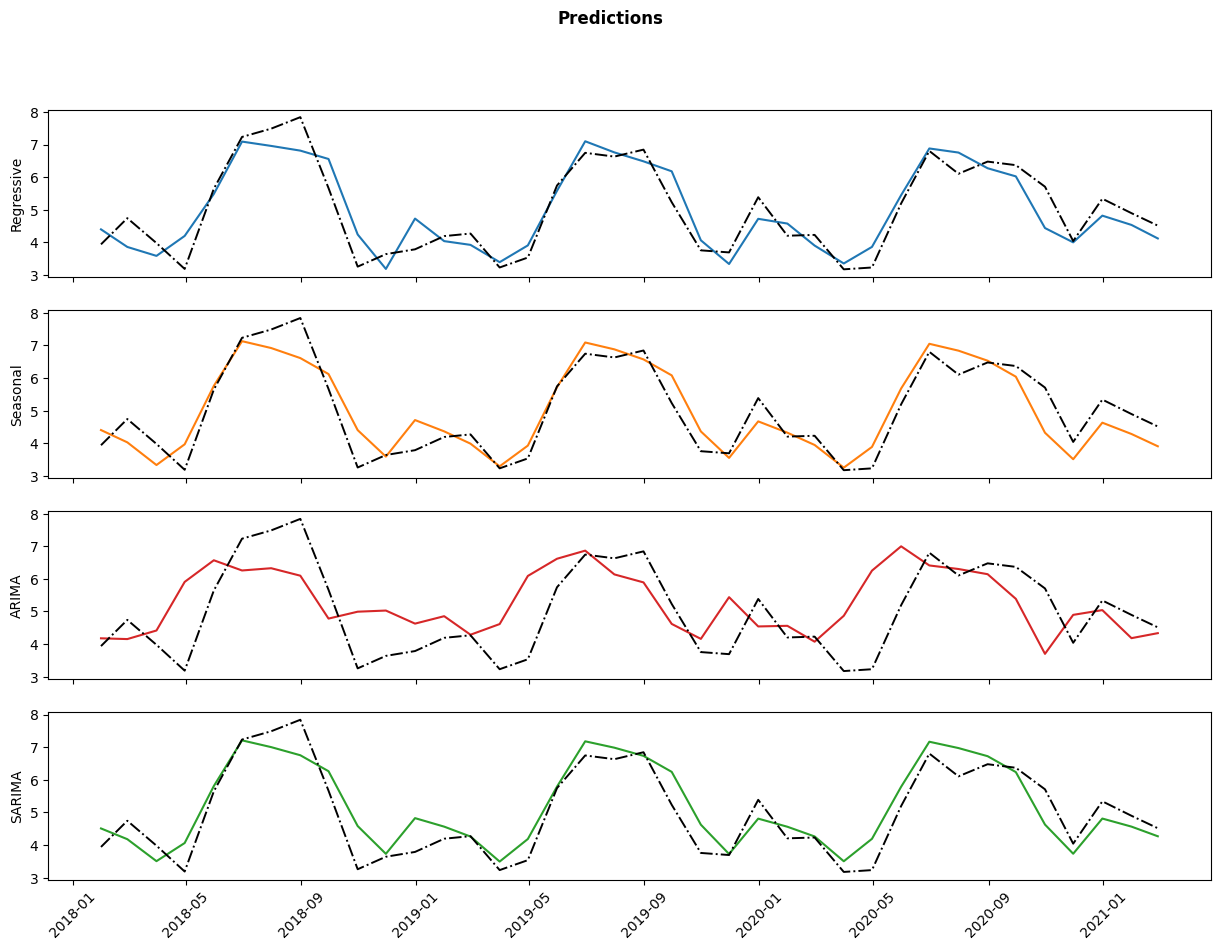
\includegraphics[width=1.00\textwidth]{./images/tiru/monthlyPred.png}
\end{center}

The similar nature of the residuals and their distributions confirms the same.

\begin{center}
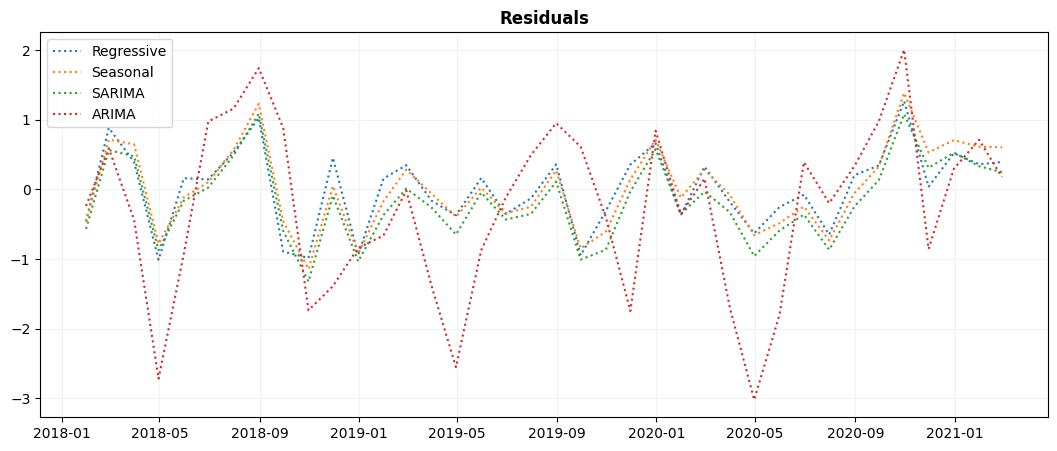
\includegraphics[width=1.00\textwidth]{./images/tiru/monthlyResid.png}
\end{center}

\begin{center}
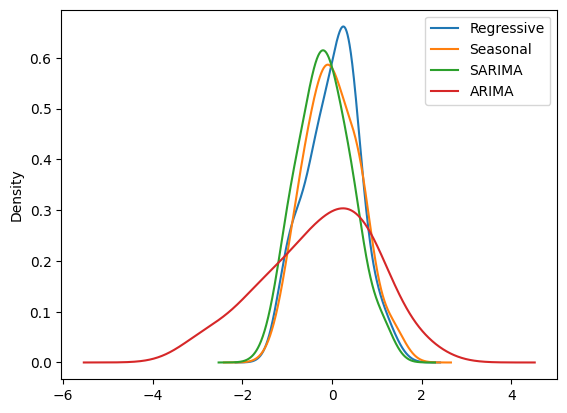
\includegraphics[width=0.8\linewidth]{./images/tiru/monthlyDist.png}
\end{center}

The Q-Q plots for all the models don't closely follow the ideal line, maybe due to lack of data points or because of the non-stationary nature of the series.

\begin{center}
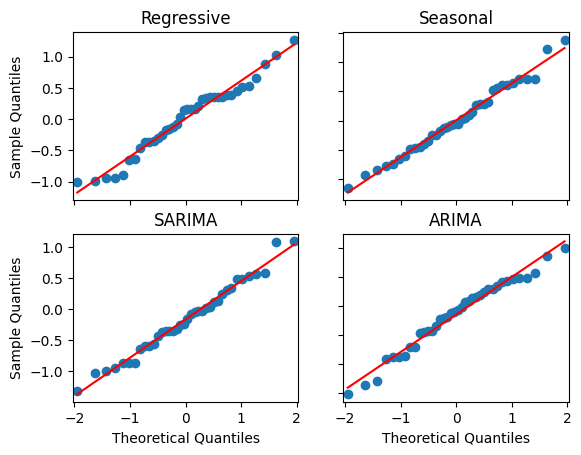
\includegraphics[width=0.8\linewidth]{./images/tiru/monthlyQQ.png}
\end{center}
\pagebreak

\subsubsection{Weekly}
\label{sec:org76b144b}
Now let's take a look at the \texttt{decomposition} of the weekly wind speed data, again the pattern repeats, seasonal data with large and small spikes and no clear trend.

\begin{figure}[htbp]
\centering
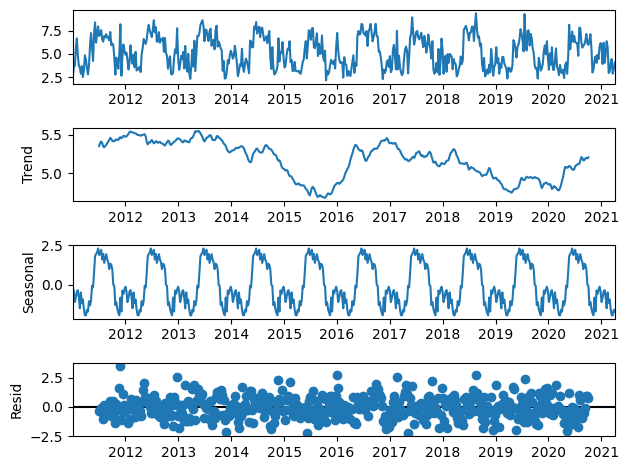
\includegraphics[width=1.0\textwidth]{./images/tiru/weeklyDecomp.png}
Weekly Wind Speed Decomposition
\end{figure}

The decomposed components for the Regressive and Seasonal DLM models are fitted, they show similar trend and seasonal variations.

\begin{center}
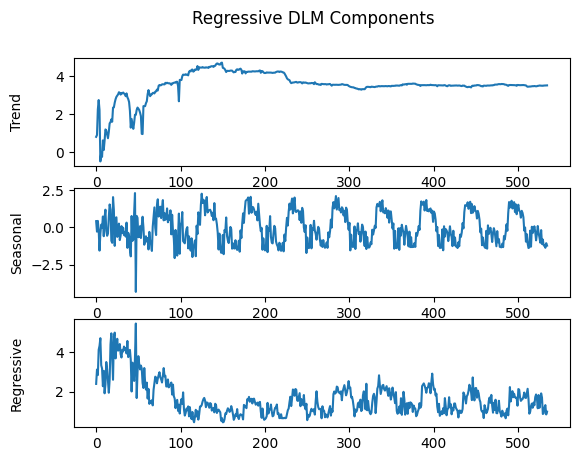
\includegraphics[width=0.45\linewidth]{./images/tiru/weeklyRegDecomp.png}
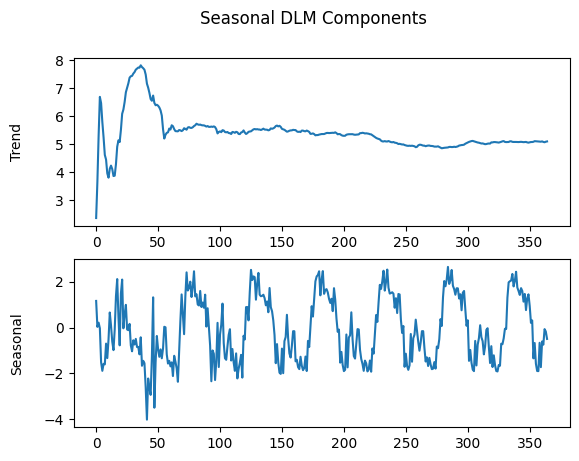
\includegraphics[width=0.45\linewidth]{./images/tiru/weeklySeasDecomp.png}
\end{center}

Looking at the predictions for the various models, both ARIMA and SARIMA perform quite poorly in comparison to the two DLM models.

\begin{center}
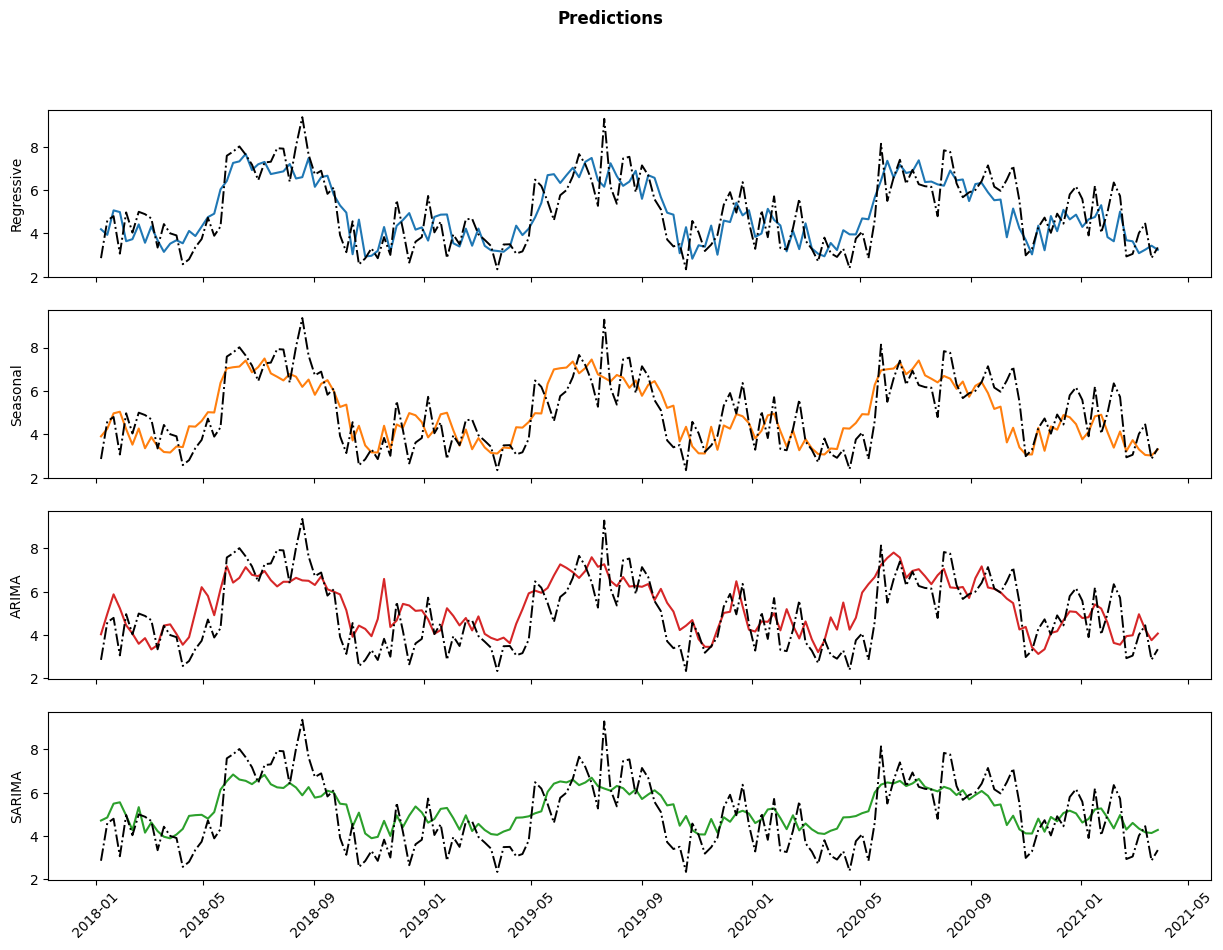
\includegraphics[width=1.00\textwidth]{./images/tiru/weeklyPred.png}
\end{center}

However because of the large number of data points, the residuals don't show any clear information but their distribution suggests normality.

\begin{center}
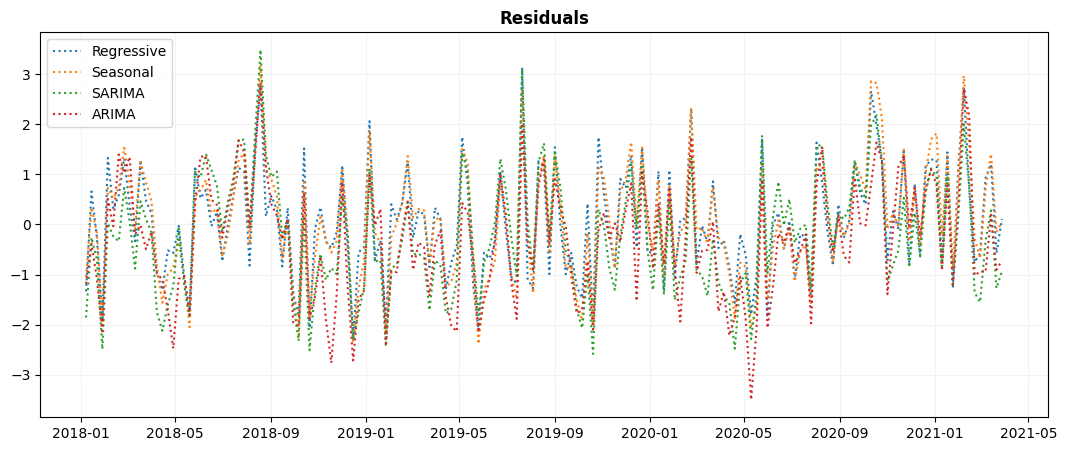
\includegraphics[width=1.00\textwidth]{./images/tiru/weeklyResid.png}
\end{center}

\begin{center}
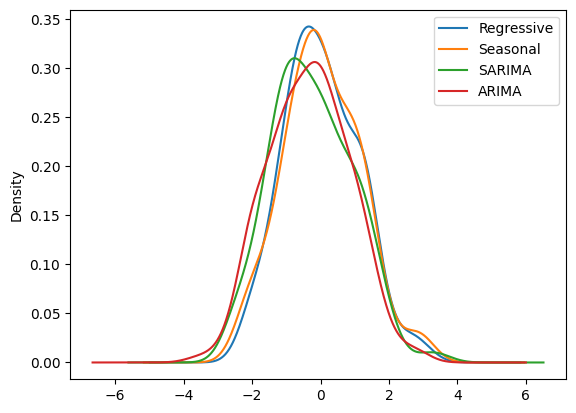
\includegraphics[width=0.8\linewidth]{./images/tiru/weeklyDist.png}
\end{center}

The Q-Q plots reinforce the same suggestion, for all the models they follow the \emph{y = x} line.

\begin{center}
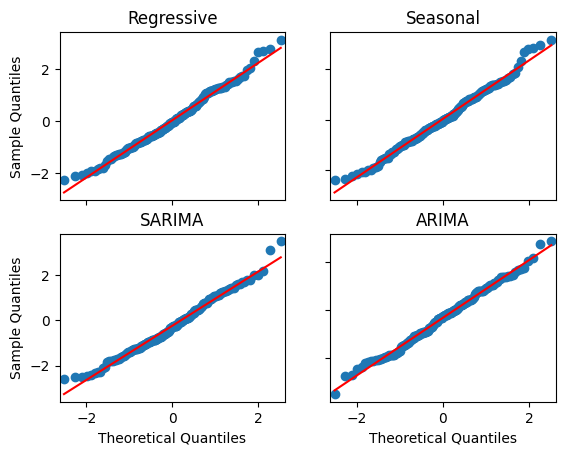
\includegraphics[width=0.8\linewidth]{./images/tiru/weeklyQQ.png}
\end{center}

\pagebreak
\subsubsection{Daily}
\label{sec:org8401fdc}
Looking at the \texttt{decomposition} of the daily wind-speed data, there's not a lot one can extract from it except maybe the fact that there's periodic seasonallity.

\begin{figure}[htbp]
\centering
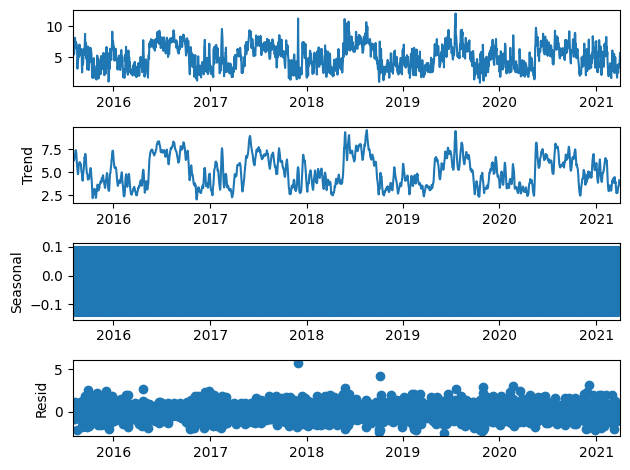
\includegraphics[width=1.0\textwidth]{./images/tiru/dailyDecomp.png}
Daily Wind Speed Decomposition
\end{figure}

Upon constructing the dynamic regressive and seasonal DLM models, their decomposed components are then fitted.

\begin{center}
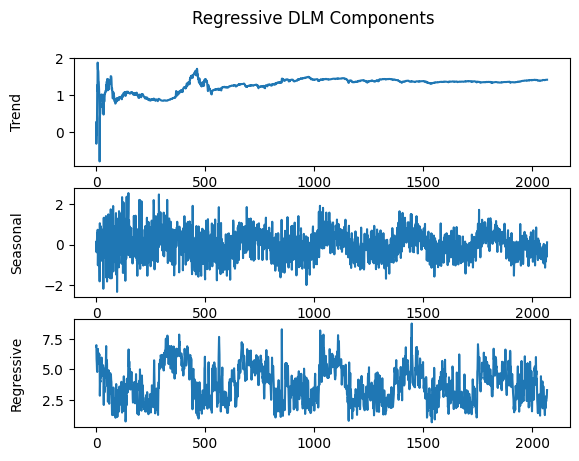
\includegraphics[width=0.45\linewidth]{./images/tiru/dailyRegDecomp.png}
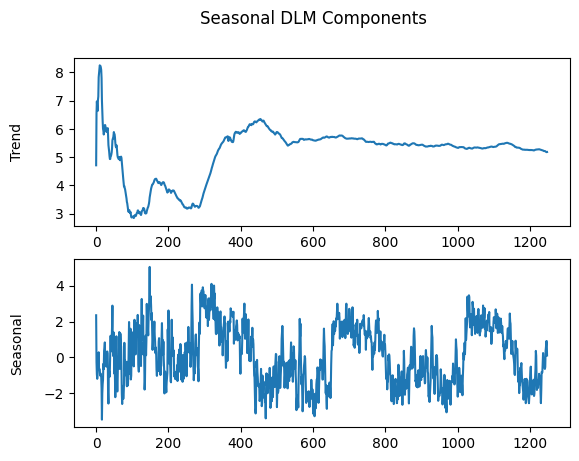
\includegraphics[width=0.45\linewidth]{./images/tiru/dailySeasDecomp.png}
\end{center}

Now, taking a look at the predictions for the various models, it's quite evident that regressive DLM model provides the best fit, this can be seen at the \texttt{2019-07} mark where there's a huge spike that only it's fitting.

\begin{center}
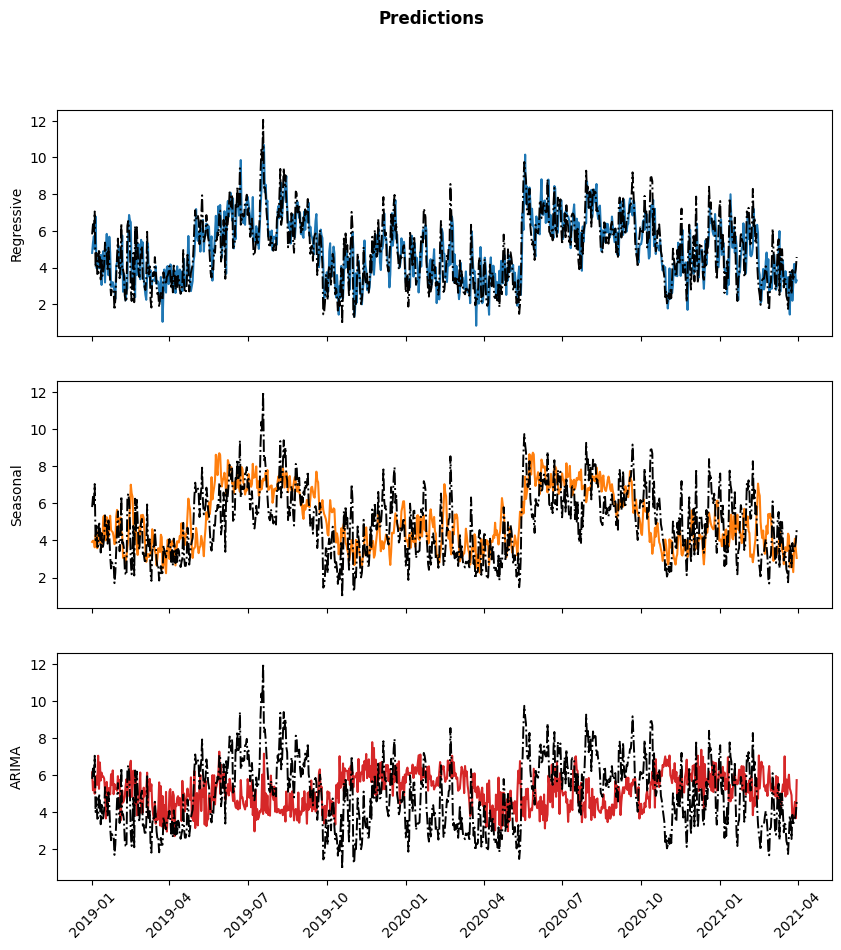
\includegraphics[width=1.00\textwidth]{./images/tiru/dailyPred.png}
\end{center}

Looking at the generated residuals and their distribution, the Regressive model has highest distribution of the residuals at a very small error value explaining its good fit.

\begin{center}
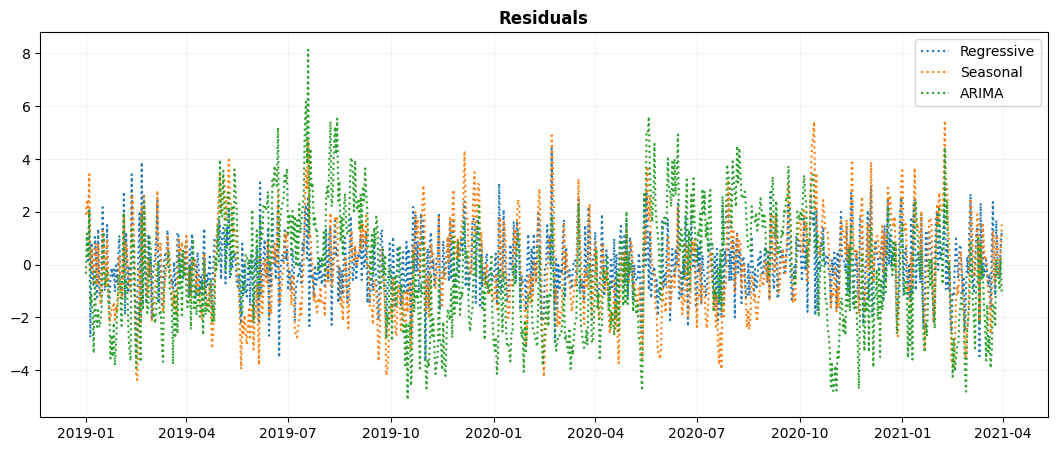
\includegraphics[width=1.00\textwidth]{./images/tiru/dailyResid.png}
\end{center}

\begin{center}
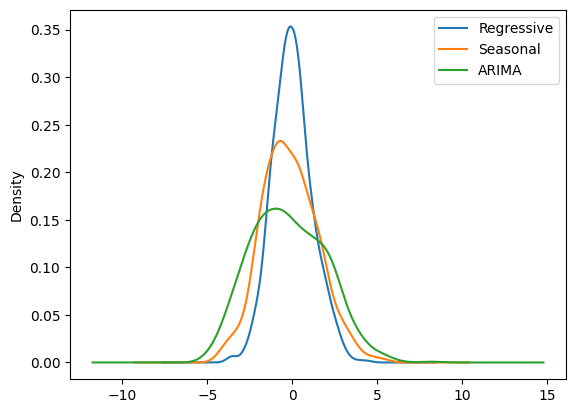
\includegraphics[width=0.8\linewidth]{./images/tiru/dailyDist.png}
\end{center}

Taking a look at the Q-Q plots, one can observe that the ARIMA model has a bit of skewness associated with its residual distribution.

\begin{center}
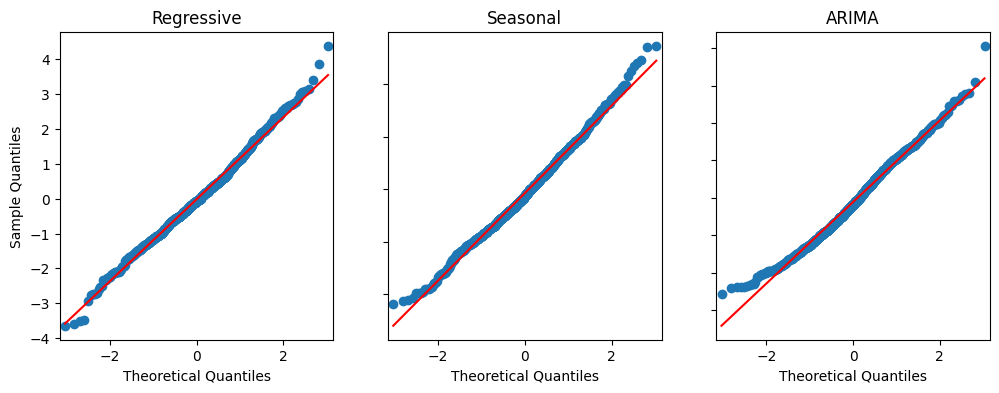
\includegraphics[width=0.8\linewidth]{./images/tiru/dailyQQ.png}
\end{center}

\pagebreak

\section{Results}
\label{sec:orgbfd2bcb}
\subsection{Bhadla}
\label{sec:org053fdd4}
\subsubsection{Monthly}
\label{sec:orgaac700a}
\begin{itemize}
\item ADF Statistic: -5.125199877123293, p-value: 1.247 \texttimes{} 10\textsuperscript{-5}
\item ARIMA Order: (1, 0, 0), SARIMA Order: (1, 0, 0), (1, 0, 2, 12)
\item Errors
\end{itemize}
\begin{center}
\begin{tabular}{lrrrr}
Error & Regressive & \textbf{Seasonal} & SARIMA & ARIMA\\[0pt]
\hline
RMSE & 26.4476 & 25.6720 & 39.6350 & 71.3908\\[0pt]
MAE & 21.8707 & 21.2476 & 33.7098 & 58.5001\\[0pt]
MAPE & 0.0372 & 0.0365 & 0.0587 & 0.0987\\[0pt]
\end{tabular}
\end{center}
\begin{itemize}
\item Shapiro-Wilk
\end{itemize}
\begin{center}
\begin{tabular}{lrrl}
Model & Statistic & p-value & Result\\[0pt]
\hline
Regressive & 0.9822 & 0.6874 & Normal\\[0pt]
Seasonal & 0.9863 & 0.8529 & Normal\\[0pt]
SARIMA & 0.9391 & 0.0164 & Not normal\\[0pt]
ARIMA & 0.9358 & 0.0124 & Not normal\\[0pt]
\end{tabular}
\end{center}
\subsubsection{Weekly}
\label{sec:orgcbe169a}
\begin{itemize}
\item ADF Statistic: -10.556604133312076, p-value: 7.923 \texttimes{} 10\textsuperscript{-19}
\item ARIMA Order: (1, 0, 0), SARIMA Order: (1, 0, 1), (1, 0, 2, 52)
\item Errors
\end{itemize}
\begin{center}
\begin{tabular}{lrrrr}
Error & \textbf{Regressive} & Seasonal & SARIMA & ARIMA\\[0pt]
\hline
RMSE & 48.4967 & 53.4963 & 56.3986 & 61.0935\\[0pt]
MAE & 38.4183 & 42.9263 & 45.7328 & 47.8263\\[0pt]
MAPE & 0.0663 & 0.0735 & 0.0786 & 0.0821\\[0pt]
\end{tabular}
\end{center}
\begin{itemize}
\item Shapiro-Wilk
\end{itemize}
\begin{center}
\begin{tabular}{lrrl}
Model & Statistic & p-value & Result\\[0pt]
\hline
Regressive & 0.9884 & 0.0924 & Normal\\[0pt]
Seasonal & 0.9855 & 0.0318 & Not Normal\\[0pt]
SARIMA & 0.9920 & 0.3185 & Normal\\[0pt]
ARIMA & 0.9910 & 0.2303 & Normal\\[0pt]
\end{tabular}
\end{center}

\subsection{Tiruvananthpuram}
\label{sec:orga4edf91}
\subsubsection{Monthly}
\label{sec:org89f8d24}
\begin{itemize}
\item ADF Statistic: -1.7364350405091447, p-value: 0.41244, not stationary
\item ARIMA Order: (1, 0, 0), SARIMA Order: (1, 0, 0), (1, 0, 2, 12)
\item Errors
\end{itemize}
\begin{center}
\begin{tabular}{lrrrr}
Error & \textbf{Regressive} & Seasonal & SARIMA & ARIMA\\[0pt]
\hline
RMSE & 0.5636 & 0.5862 & 0.5964 & 1.2335\\[0pt]
MAE & 0.4688 & 0.4774 & 0.4838 & 0.9814\\[0pt]
MAPE & 0.0993 & 0.1015 & 0.0980 & 0.1849\\[0pt]
\end{tabular}
\end{center}
\begin{itemize}
\item Shapiro-Wilk
\end{itemize}
\begin{center}
\begin{tabular}{lrrl}
Model & Statistic & p-value & Result\\[0pt]
\hline
Regressive & 0.9663 & 0.3031 & Normal\\[0pt]
Seasonal & 0.9830 & 0.8202 & Normal\\[0pt]
SARIMA & 0.9820 & 0.7877 & Normal\\[0pt]
ARIMA & 0.9717 & 0.4406 & Normal\\[0pt]
\end{tabular}
\end{center}
\subsubsection{Weekly}
\label{sec:org23dda29}
\begin{itemize}
\item ADF Statistic: -6.4586325869970445, p-value: 1.462 \texttimes{} 10\textsuperscript{-8}
\item ARIMA Order: (1, 0, 1), SARIMA Order: (1, 0, 1), (1, 0, 2, 52)
\item Errors
\end{itemize}
\begin{center}
\begin{tabular}{lrrrr}
Error & \textbf{Regressive} & Seasonal & SARIMA & ARIMA\\[0pt]
\hline
RMSE & 1.0835 & 1.1327 & 1.1986 & 1.2137\\[0pt]
MAE & 0.8795 & 0.9031 & 0.9905 & 0.9822\\[0pt]
MAPE & 0.1892 & 0.1927 & 0.1939 & 0.1909\\[0pt]
\end{tabular}
\end{center}
\begin{itemize}
\item Shapiro-Wilk
\end{itemize}
\begin{center}
\begin{tabular}{lrrl}
Model & Statistic & p-value & Result\\[0pt]
\hline
Regressive & 0.9886 & 0.1917 & Normal\\[0pt]
Seasonal & 0.9898 & 0.2668 & Normal\\[0pt]
SARIMA & 0.9863 & 0.0982 & Normal\\[0pt]
ARIMA & 0.9941 & 0.7373 & Normal\\[0pt]
\end{tabular}
\end{center}
\subsubsection{Daily}
\label{sec:org6a059fe}
\begin{itemize}
\item ADF Statistic: -4.12281187307635,  p-value: 8.887 \texttimes{} 10\textsuperscript{-4}
\item ARIMA Order: (0, 0, 1)
\item Errors
\end{itemize}
\begin{center}
\begin{tabular}{lrrr}
Error & \textbf{Regressive} & Seasonal & ARIMA\\[0pt]
\hline
RMSE & 1.1719 & 1.6634 & 2.1902\\[0pt]
MAE & 0.9186 & 1.3385 & 1.8171\\[0pt]
MAPE & 0.2103 & 0.2824 & 0.3631\\[0pt]
\end{tabular}
\end{center}
\begin{itemize}
\item Shapiro-Wilk
\end{itemize}
\begin{center}
\begin{tabular}{lrrl}
Model & Statistic & p-value & Result\\[0pt]
\hline
Regressive & 0.9949 & 0.0080 & Not normal\\[0pt]
Seasonal & 0.9940 & 0.0024 & Not normal\\[0pt]
ARIMA & 0.9898 & 1.7\texttimes{}10\textsuperscript{-5} & Not normal\\[0pt]
\end{tabular}
\end{center}
\subsection{Conclusion}
\label{sec:org728f62a}
Except for monthly resampled wind speed data for Tiruvananthapuram, all the other time series were stationary. Because of the non-stationary nature of that data, ARIMA predictions for it were starkly inaccurate compared to other models. On all the other cases including this one, DLM models outshone their (S)ARIMA rivals. Regressive DLM model performed well in all cases except the Monthly GHI predictions for Bhadla where seasonal DLM model was a bit better.

Coming to the normality analysis of the residuals, the residuals for ARIMA and SARIMA didn't follow a gaussian distribution in the case of Monthly GHI forecast which can be attributed to poor modeling or overfitting. This is also corroborated by looking at the Q-Q plots which don't really follow the \emph{y = x} line for those cases. When it came to daily wind speed predictions however, all the three models (Regressive, Seasonal and ARIMA) didn't fit a normal distribution and failed the Shapiro-Wilk test.

This can however be explained by the fact that for daily data, the number of data points is large and Shapiro-Wilk test doesn't perform well under those circumstances. This fact is reflected in the daily wind speed analysis for the other locations as well as all of them fail the test too. However, looking at the Q-Q plot for the daily wind speed data, we can see that for the most part, the residual do exhibit normal characteristics.
\section{Future Work}
\label{sec:orgacdd32e}
For the analysis of daily data, the comparison was done only between ARIMA and the DLM models, because of the nature of SARIMA models and the computation cost associated with it, it could not be performed. That is something which one can look into for comparing the advantages, if any that DLM models might hold over SARIMA models, one cannot say for sure. They performed better in weekly and daily analysis though in our limited testing. There's also scope for improving the DLM models by incorporating auto-regressive components that go beyond one value lag.
\pagebreak
\section{Appendix}
\label{sec:org660708f}
\subsection{Bhopal}
\label{sec:org81224bf}
\begin{center}
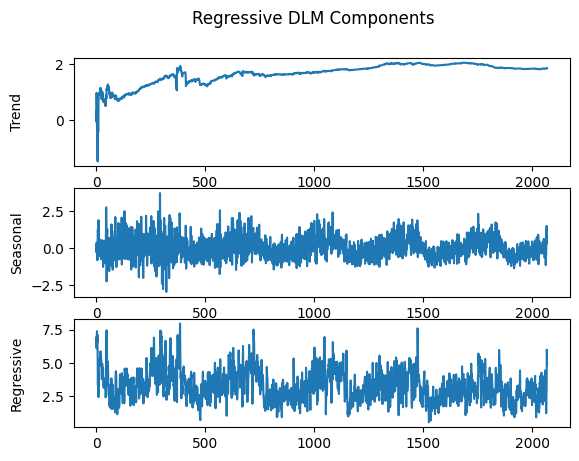
\includegraphics[width=0.45\linewidth]{./images/bhopal/reg.png}
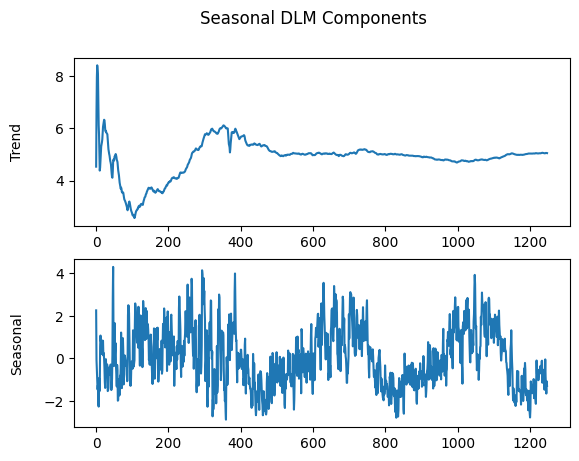
\includegraphics[width=0.45\linewidth]{./images/bhopal/seas.png}
\end{center}

\begin{center}
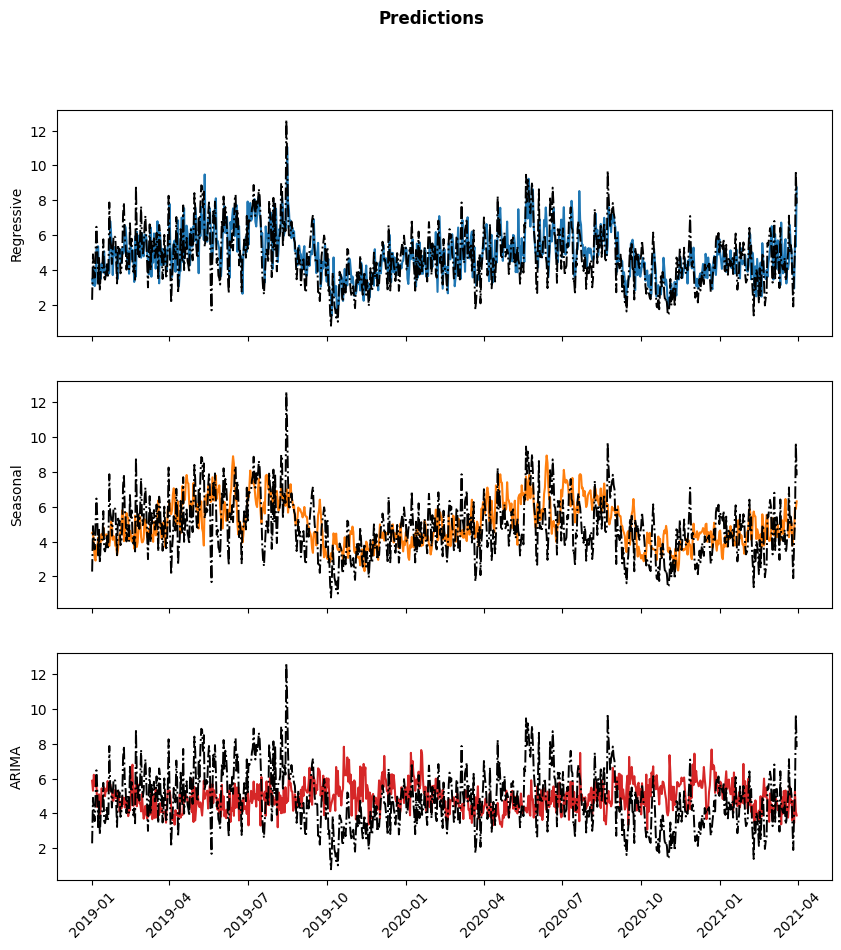
\includegraphics[width=0.9\textwidth]{./images/bhopal/pred.png}
\end{center}

ARIMA performs quite poorly (1.89 RMSE) compared to the other two DLM models (1.30 and 1.64 RMSE).

\begin{center}
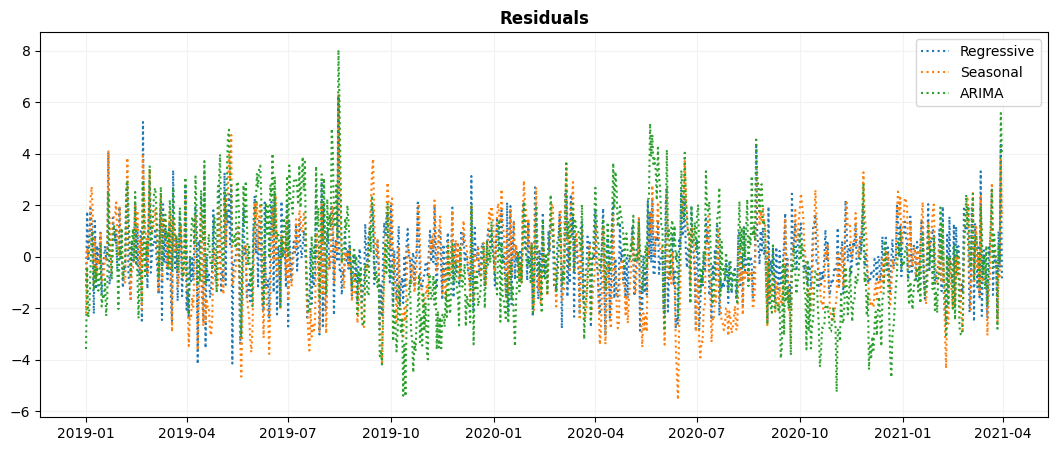
\includegraphics[width=1.00\textwidth]{./images/bhopal/resid.png}
\end{center}

\begin{center}
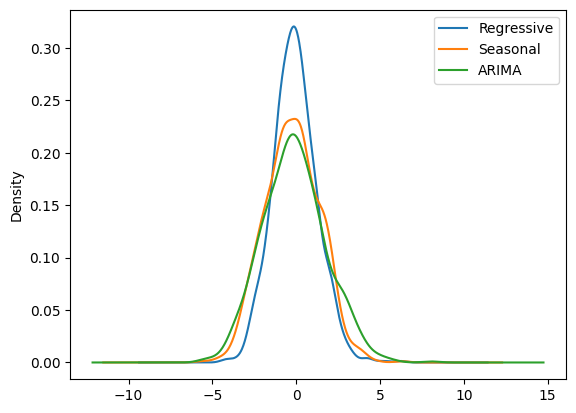
\includegraphics[width=0.8\linewidth]{./images/bhopal/dist.png}
\end{center}

\begin{center}
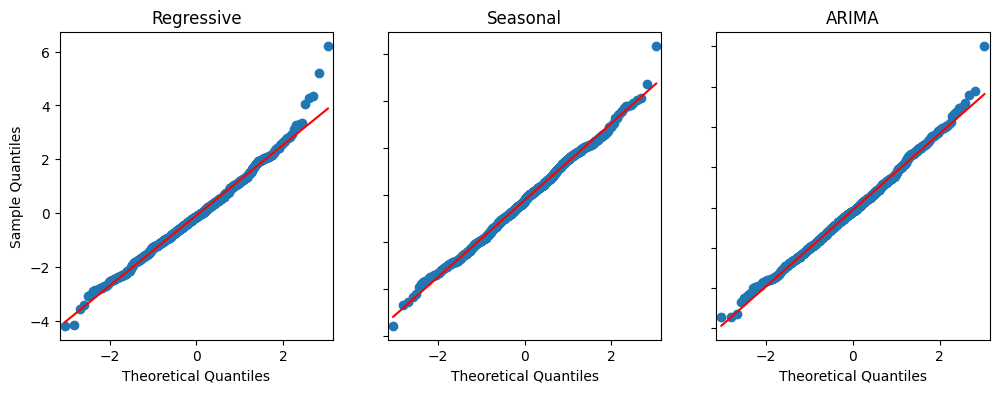
\includegraphics[width=0.8\linewidth]{./images/bhopal/qq.png}
\end{center}

\pagebreak

\subsection{Hamirpur}
\label{sec:org5400ece}
\begin{center}
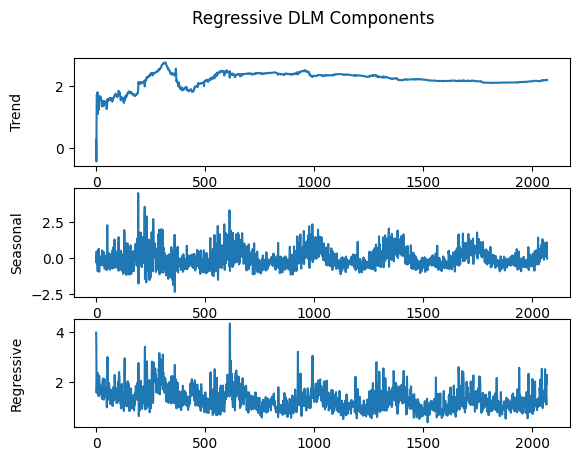
\includegraphics[width=0.45\linewidth]{./images/hamirpur/reg.png}
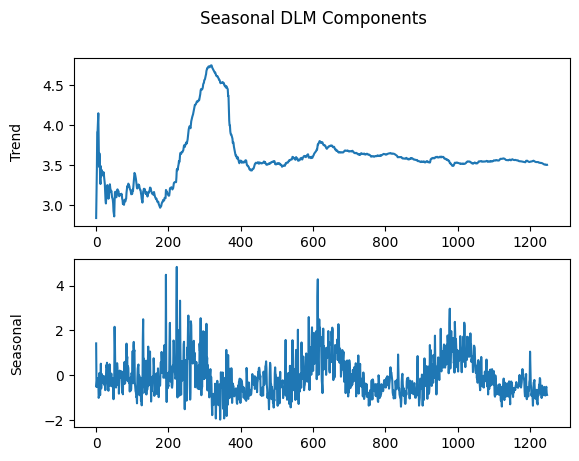
\includegraphics[width=0.45\linewidth]{./images/hamirpur/seas.png}
\end{center}

\begin{center}
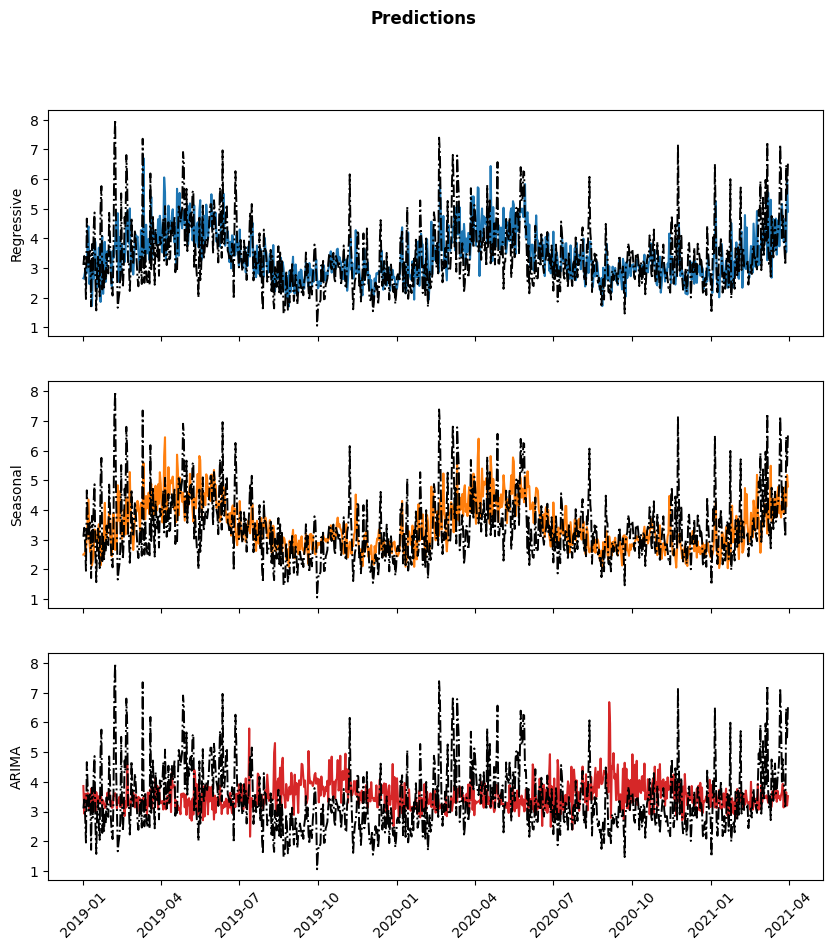
\includegraphics[width=0.9\textwidth]{./images/hamirpur/pred.png}
\end{center}

The sudden dips and rises in the data are not very well modelled by the ARIMA model and the DLM models fail to account for the outlying rises. The RMSE values for the Regressive, Seasonal and ARIMA models are 1.036, 1.110 and 1.251 respectively.

\begin{center}
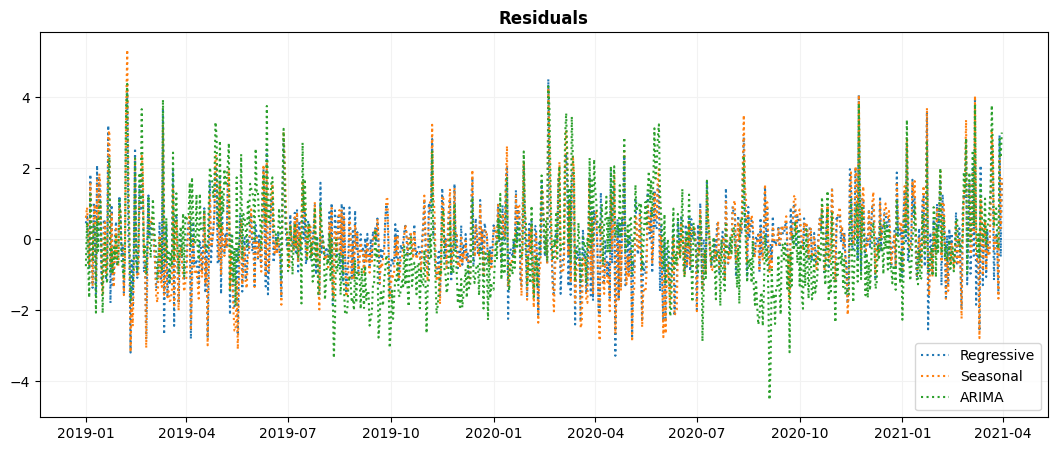
\includegraphics[width=1.00\textwidth]{./images/hamirpur/resid.png}
\end{center}

\begin{center}
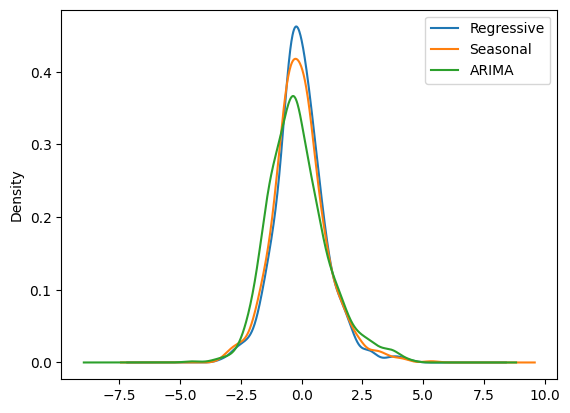
\includegraphics[width=0.8\linewidth]{./images/hamirpur/dist.png}
\end{center}

All three models fail the Shapiro-Wilk test and it is supported by the Q-Q plots too, all the models deviate quite a bit from the y=x line.

\begin{center}
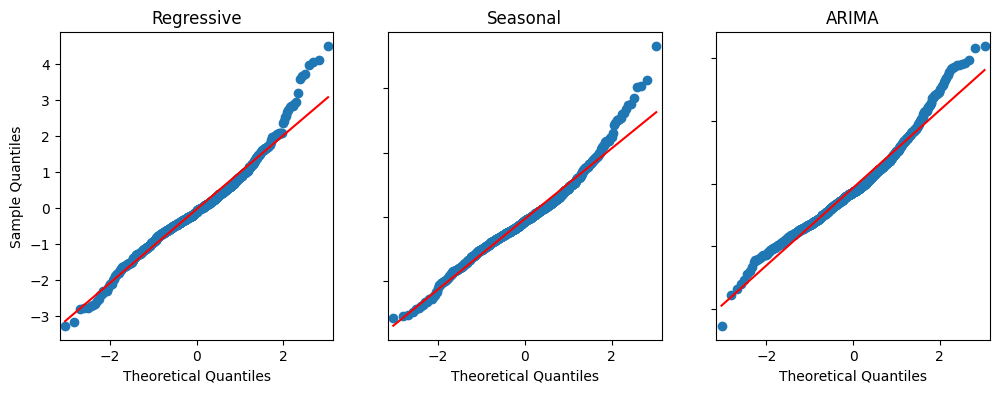
\includegraphics[width=0.8\linewidth]{./images/hamirpur/qq.png}
\end{center}

\pagebreak

\subsection{Jafrabad}
\label{sec:org7f10659}
\begin{center}
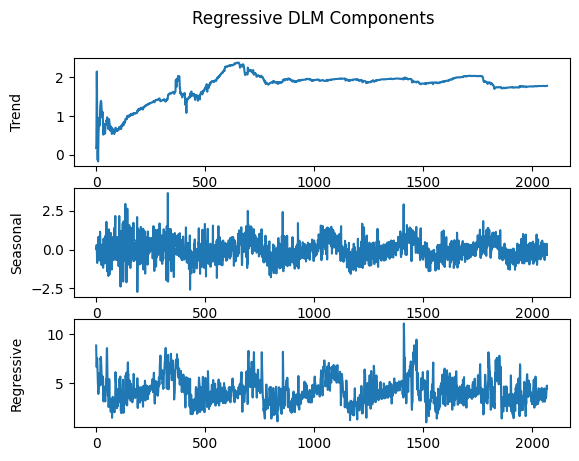
\includegraphics[width=0.45\linewidth]{./images/jafrabad/reg.png}
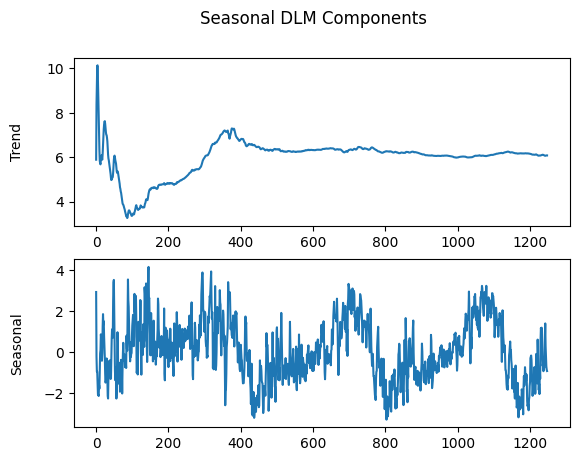
\includegraphics[width=0.45\linewidth]{./images/jafrabad/seas.png}
\end{center}

\begin{center}
\includegraphics[width=0.9\textwidth]{./images/jafrabad/pred.png}
\end{center}

There are two interesting regions of concern, July 2019 and 2020 where there's a sudden change in the underlying data pattern which only the regressive model correctly fits. Hence its RMSE (1.27) is quite low compared to Seasonal DLM (1.83) and the ARIMA model(2.16).

\begin{center}
\includegraphics[width=1.00\textwidth]{./images/jafrabad/resid.png}
\end{center}

\begin{center}
\includegraphics[width=0.8\linewidth]{./images/jafrabad/dist.png}
\end{center}

All three models fail the Shapiro-Wilk test and it is supported by the Q-Q plots too, all the models deviate quite a bit from the y=x line.

\begin{center}
\includegraphics[width=0.8\linewidth]{./images/jafrabad/qq.png}
\end{center}

\section{Bibliography}
\label{sec:org06d47f6}
\begin{enumerate}
\item Petris, G., Petrone, S., \& Campagnoli, P. (2009). Dynamic Linear Models with R. Springer Science \& Business Media.
\item West, M., \& Harrison, J. (1997). Bayesian forecasting and dynamic models (2nd ed.). Springer.
\item Hyndman, R.J., \& Athanasopoulos, G. (2021) Forecasting: principles and practice, 3rd edition, OTexts: Melbourne, Australia. OTexts.com/fpp3.
\item Harvey, A. C. (1990). Forecasting, structural time series models and the Kalman filter.
\item Schmidt, Alexandra M., and Hedibert F. Lopes. (2019). Dynamic models. Handbook of environmental and ecological statistics. Chapman and Hall/CRC, 2019. 57-80.
\item Cogley, T., \& Sargent, T. J. (2005). Drifts and volatilities: Monetary policies and outcomes in the post WWII US. Review of Economic Dynamics, 8(2), 262-302.
\item Liu, L., Ji, Q., \& Zhao, Z. (2019). Forecasting bitcoin returns using dynamic linear models with stochastic volatility. Journal of Forecasting, 38(2), 97-108.
\item Primiceri, G. E. (2005). Time varying structural vector autoregressions and monetary policy. Review of Economic Studies, 72(3), 821-852.
\item Chan, J. C., \& Koop, G. (2013). Modeling breaks in the monetary transmission process. Journal of Business \& Economic Statistics, 31(2), 159-170.
\item Yang, H., Guo, X., \& Yu, J. (2018). A dynamic linear model for short-term solar power forecasting. Applied Energy, 210, 1233-1243.
\item Wang, Hao, et al. (2019). Modeling and forecasting of temperature-induced strain of a long-span bridge using an improved Bayesian dynamic linear model. Engineering Structures 192 (2019): 220-232.
\item Khan, Firdos, et al. (2021). Forecasting daily new infections, deaths and recovery cases due to COVID-19 in Pakistan by using Bayesian Dynamic Linear Models. Plos one 16.6 (2021): e0253367.
\item Jiang, Y., Chen, X., \& Wu, J. (2019). A novel dynamic linear model control strategy for a linear motor. IEEE Transactions on Industrial Electronics, 66(4), 2894-2904.
\item Wang, Y. (2017). Bayesian-based Methodology for Progressive Structural Health Evaluation and Prediction by Use of Monitoring Data.
\item Ho, Siu Lau, and Min Xie. (1998). The use of ARIMA models for reliability forecasting and analysis. Computers \& industrial engineering 35.1-2 (1998): 213-216.
\item Nobre, Flávio Fonseca, et al. (2001). Dynamic linear model and SARIMA: a comparison of their forecasting performance in epidemiology. Statistics in medicine 20.20 (2001): 3051-3069.
\item Sarita Sheoran, Sumanta Pasari; Efficacy and application of the window-sliding ARIMA for daily and weekly wind speed forecasting. Journal of Renewable and Sustainable Energy 1 September 2022; 14 (5): 053305.
\item Nobre, Flávio Fonseca, et al. (2001). Dynamic linear model and SARIMA: a comparison of their forecasting performance in epidemiology. Statistics in medicine 20.20 (2001): 3051-3069.
\item \href{http://lalas.github.io/quantitativeThoughts/r/2014/09/01/dlmTutorial.html}{Nagi, A. (2014, September 1). Linear State Space Linear Models, and Kalman Filters.} (Accessed on 10\textsuperscript{th} May, 2023)
\item \href{https://pydlm.github.io/index.html}{PyDLM — PyDLM 0.1.1 documentation. (n.d.).} (Accessed on 10\textsuperscript{th} May, 2023)
\end{enumerate}
\pagebreak
\end{document}